\documentclass[notes]{beamer}       % print frame + notes
% \documentclass[notes=only]{beamer}   % only notes
% \documentclass{beamer}              % only frames

% setting
\usepackage[labelformat=empty]{caption}
% \captionsetup{labelformat=empty}
% \usepackage{xcolor}
\usepackage{color}


\title{Free software Free society}
\author{Azzam Syawqi Aziz}
\date{November 11, 2017}

\usetheme{metropolis} 

\begin{document}
\maketitle

% 1
% \note{anyone know FS ?.}
\begin{frame}
  % \frametitle{}
  \begin{center}
    \Huge Free Software ?
  \end{center}
\end{frame}

% 2
\begin{frame}
  % \frametitle{}
  \begin{center}
    \Huge Open Source ?
  \end{center}
\end{frame}

% 3
\begin{frame}
  % \frametitle{}
  \begin{center}
    \Huge Linux ? \\
    \Huge GNU ?
  \end{center}
\end{frame}

% 4
\begin{frame}
  % \frametitle{}
  \begin{center}
    \Huge Free Software {$\neq$}  Open Source \\
    \Huge GNU {$\neq$} Linux
  \end{center}
\end{frame}

\begin{frame}
  % \frametitle{}
  \begin{center}
    \Huge Libre, Bebas {$\neq$}  Gratis
  \end{center}
\end{frame}


\begin{frame}
  % \frametitle{}
  \begin{figure}
    \centering
    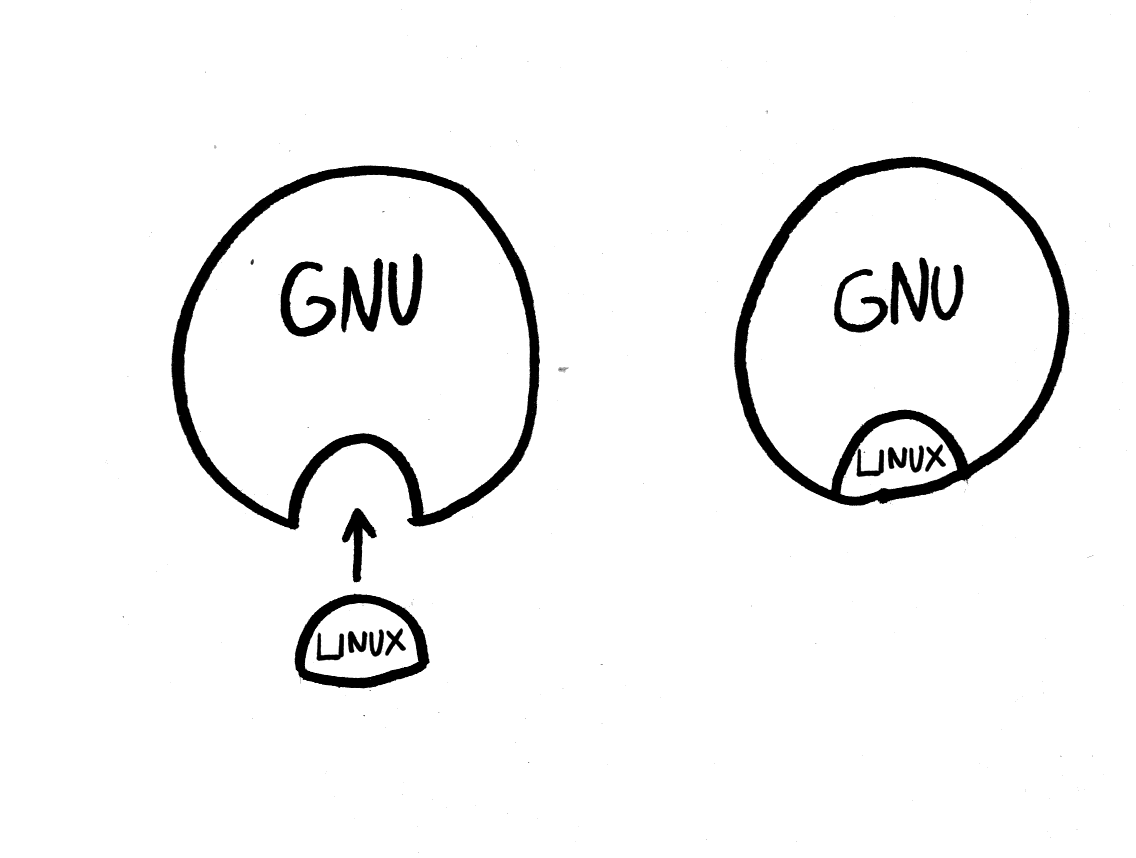
\includegraphics[scale=0.7]{gnu+linux}
    % {\transparent{0.4}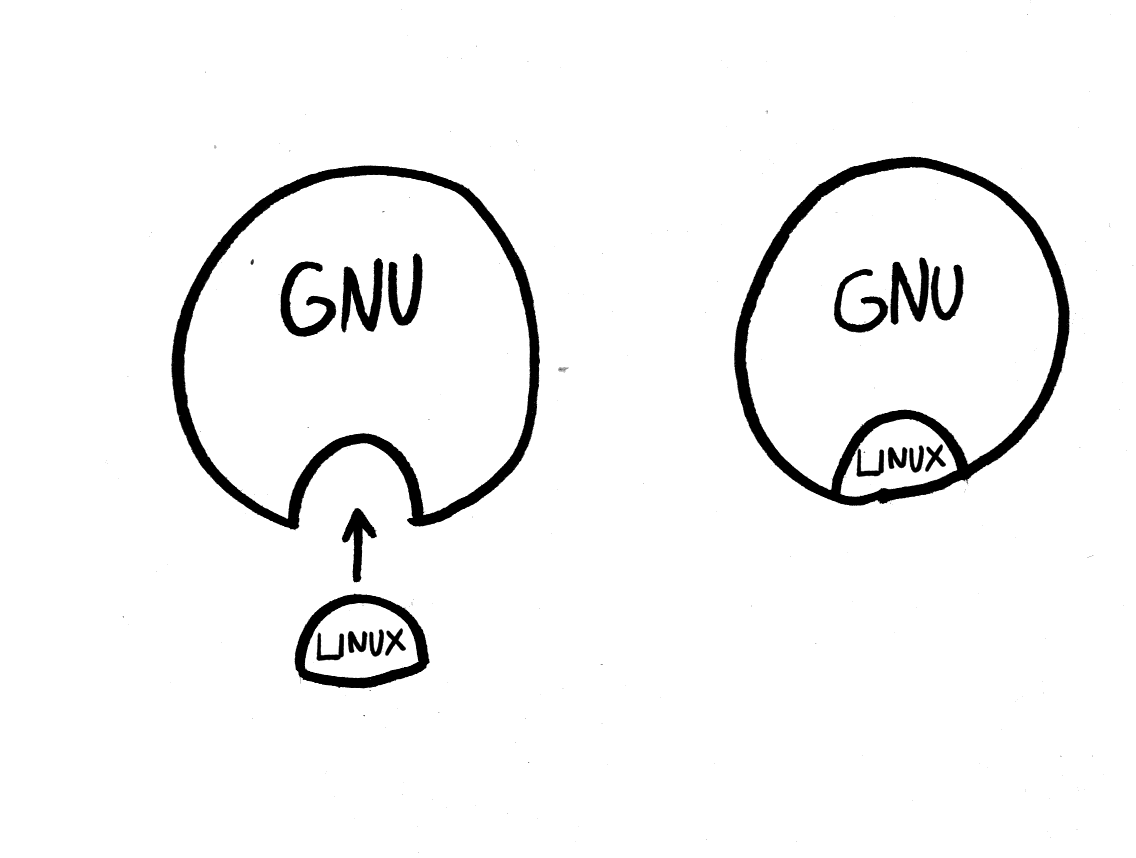
\includegraphics[width=0.5\textwidth]{gnu+linux}}%
    % \caption{}
  \end{figure}
\end{frame}

% 5
\begin{frame}
  % \frametitle{}
  \begin{center}
    \Huge Untuk sesi ini \\
    \small kita anggap keduanya sama
  \end{center}
\end{frame}

\begin{frame}
  % \frametitle{}
  \begin{center}
    \Huge Free Culture \\
    \small Masyarakat dan budaya saling berbagi
  \end{center}
\end{frame}


\begin{frame}
  \frametitle{Computer Universal}
  \begin{figure}
    \centering
    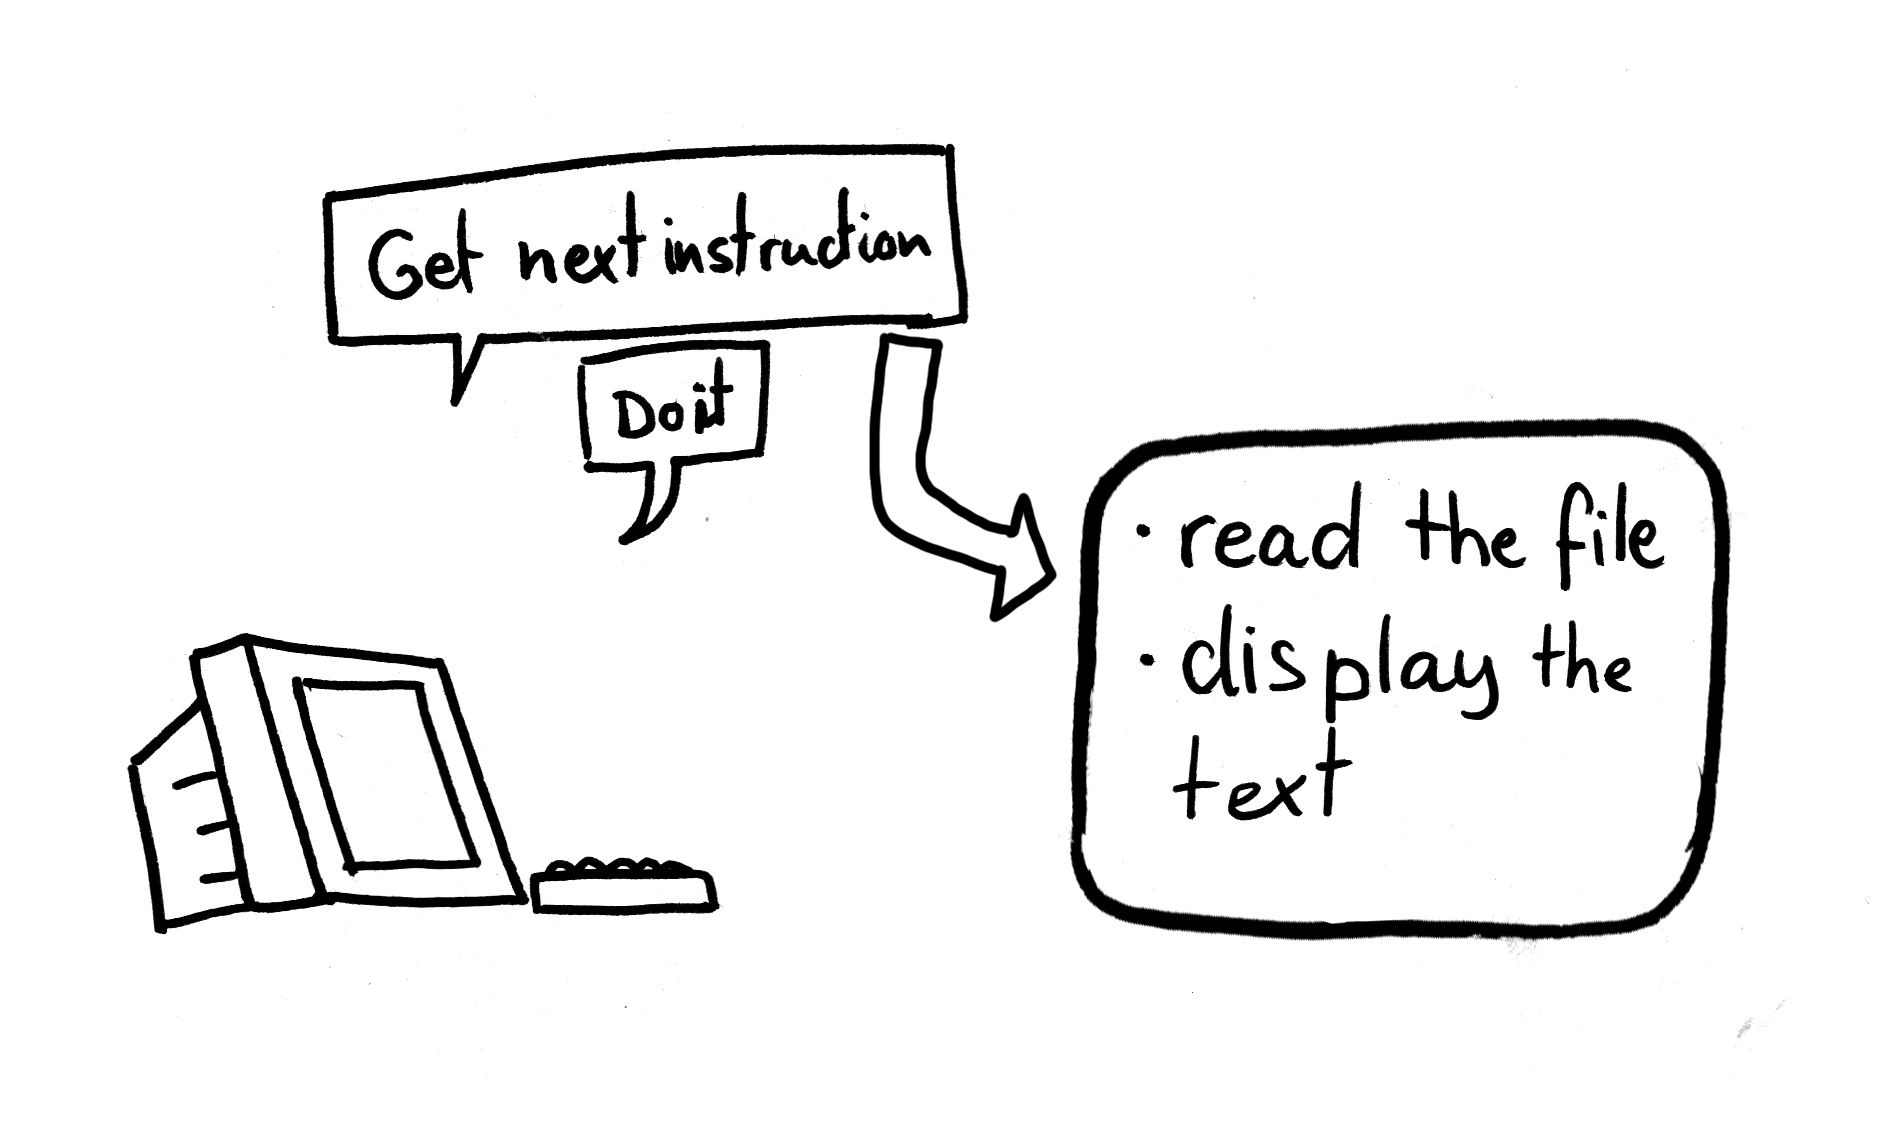
\includegraphics[scale=0.7]{what-is-comp}
  \end{figure}
\end{frame}

\begin{frame}
  \begin{figure}
    \centering
    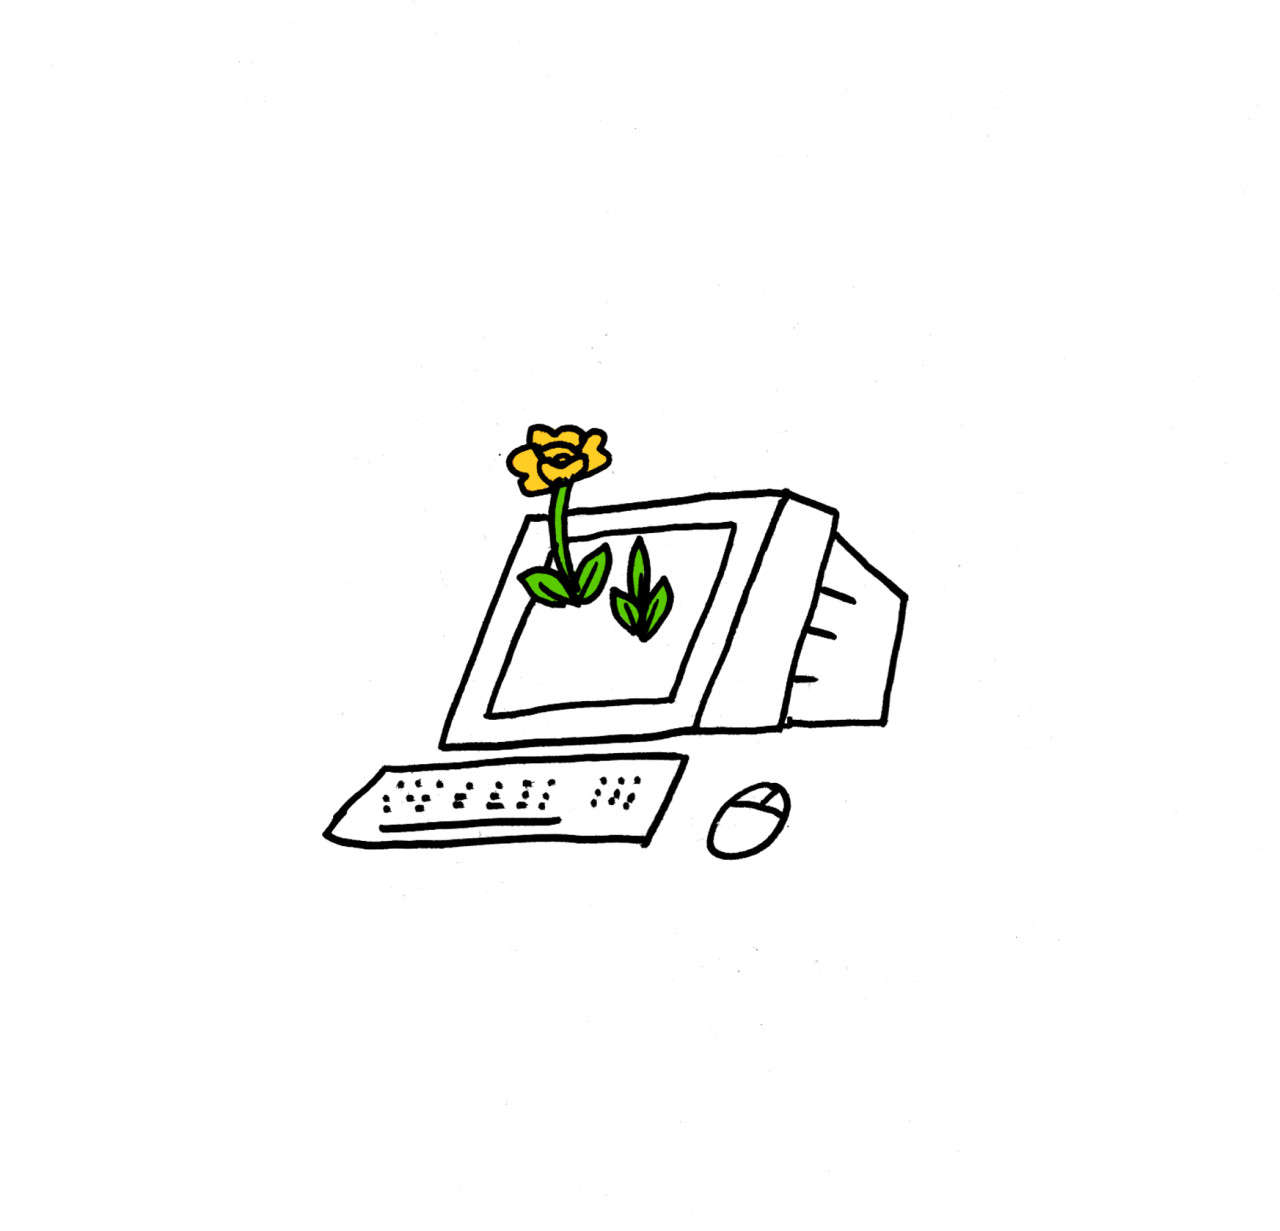
\includegraphics[scale=0.7]{comp-plants}
  \end{figure}
\end{frame}

% 3
\begin{frame}
  % \frametitle{}
  \begin{center}
    \Huge Siapa yang memberikan perintah kepada komputer kita ?
  \end{center}
\end{frame}


\begin{frame}
  \begin{figure}
    \centering
    
\includegraphics[scale=0.8]{you-comp}
  \end{figure}
\end{frame}

\begin{frame}
  \begin{figure}
    \centering
    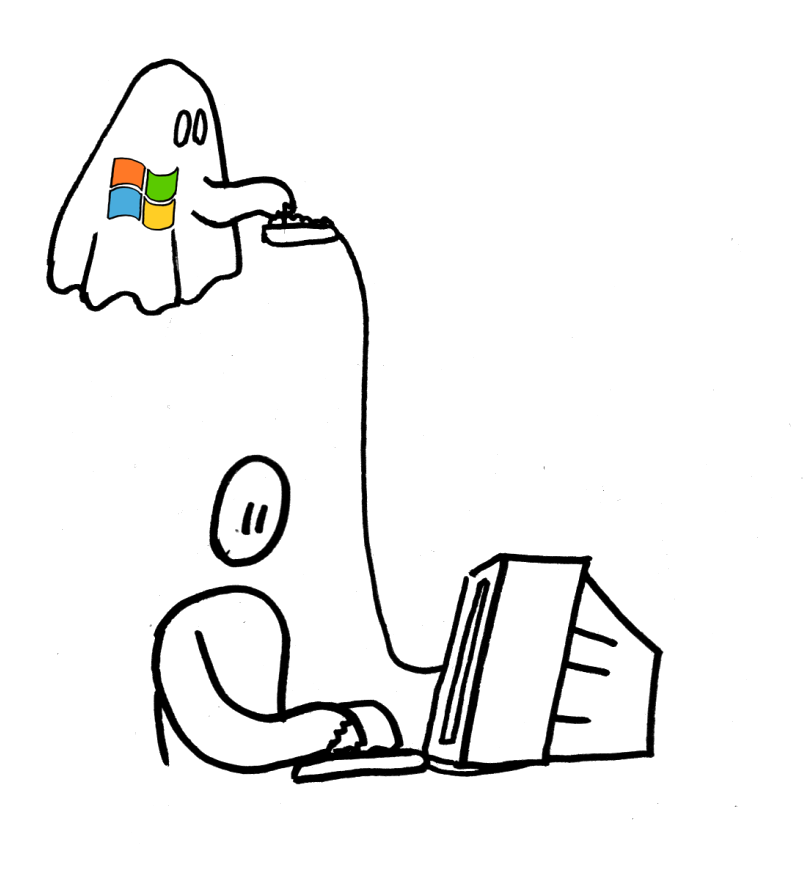
\includegraphics[scale=0.8]{ms-comp}
  \end{figure}
\end{frame}

\begin{frame}
  \begin{figure}
    \centering
    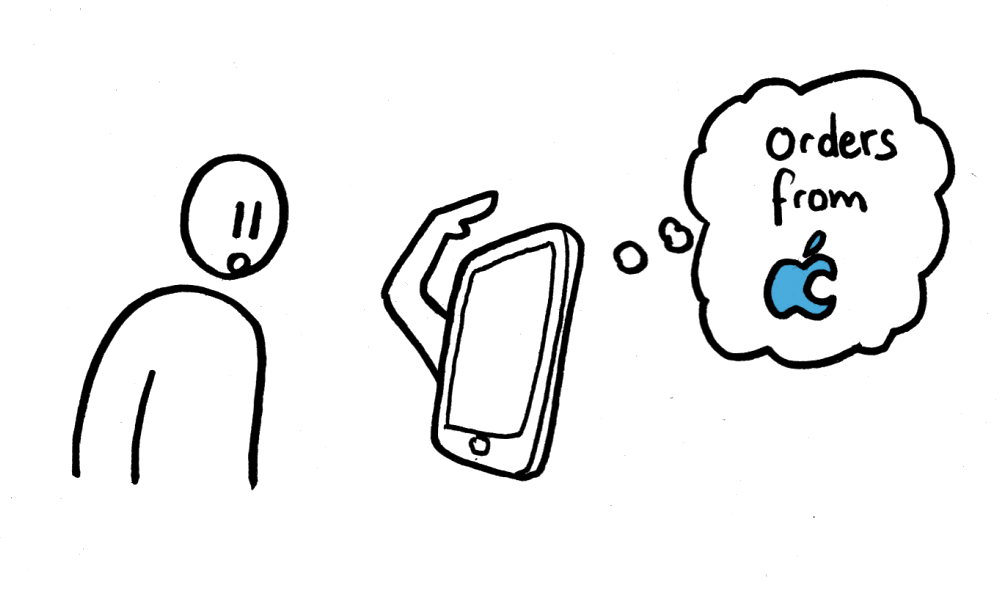
\includegraphics[scale=0.8]{apple-comp}
  \end{figure}
\end{frame}

\begin{frame}
  \begin{figure}
    \frametitle{Pengguna mengatur program}
    \centering
    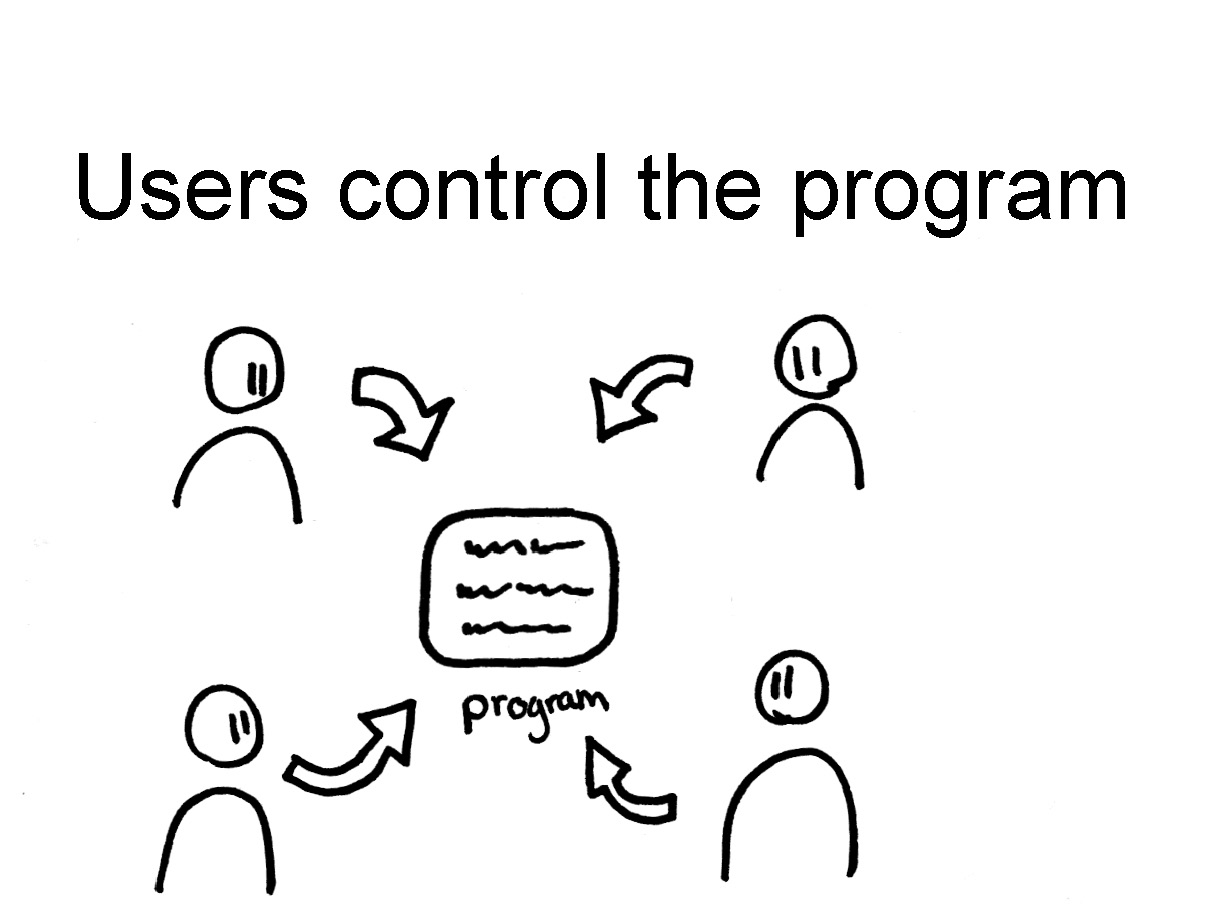
\includegraphics[scale=0.4]{user-control-program}
  \end{figure}
\end{frame}

\begin{frame}
  \begin{figure}
    \frametitle{Program mengatur user}
    \centering
    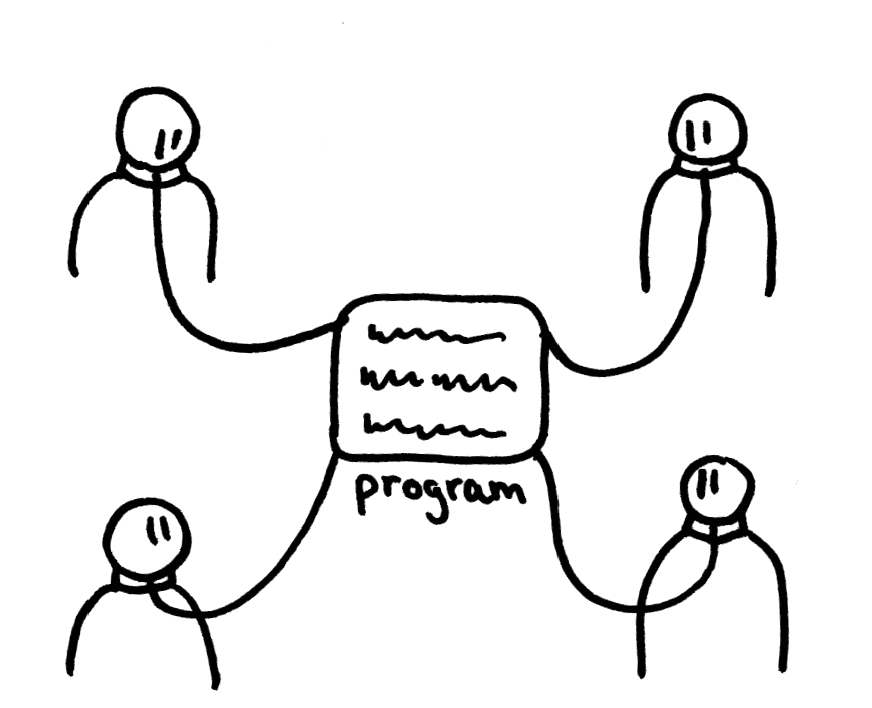
\includegraphics[scale=0.4]{program-control-user}
  \end{figure}
\end{frame}

\begin{frame}
  % \frametitle{}
  \begin{center}
    \Huge Freedom 0, 1, 2 , 3 \\
    \Large Libre, Free Software means Freedom (Kebebasan) \\
    \normalsize pikirkan tentang kebebebasan berbicara (free speech) bukan makanan gratis (free meal)
  \end{center}
\end{frame}

\begin{frame}
  \begin{figure}
    \frametitle{Kebebasan 0}
    \centering
    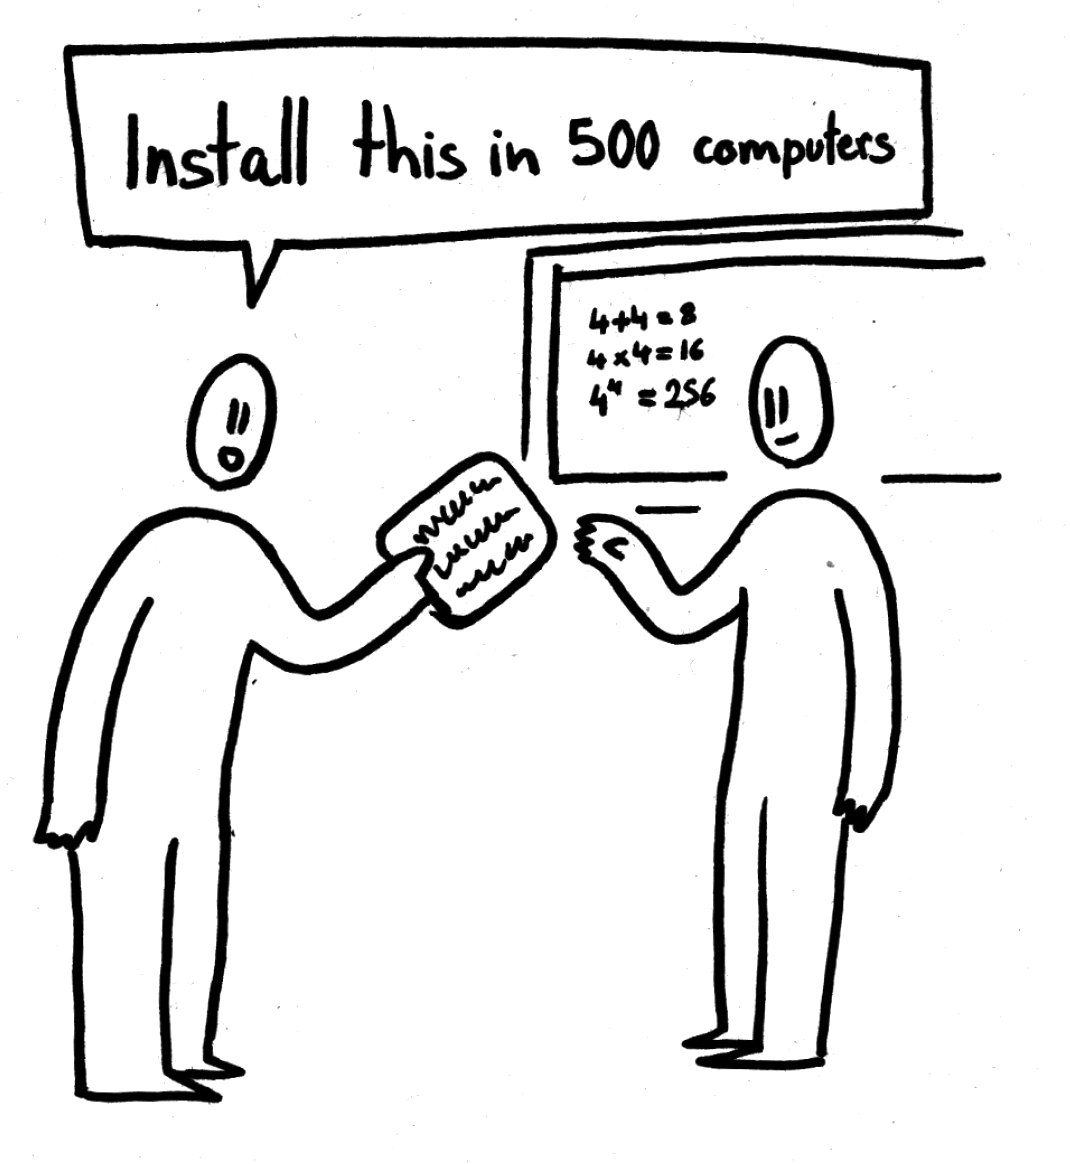
\includegraphics[scale=0.3]{fr-run}
    \caption{Freedom 0 : Menjalan program}
  \end{figure}
\end{frame}

\begin{frame}
  \begin{figure}
    \frametitle{Kebebasan 1}
    \centering
    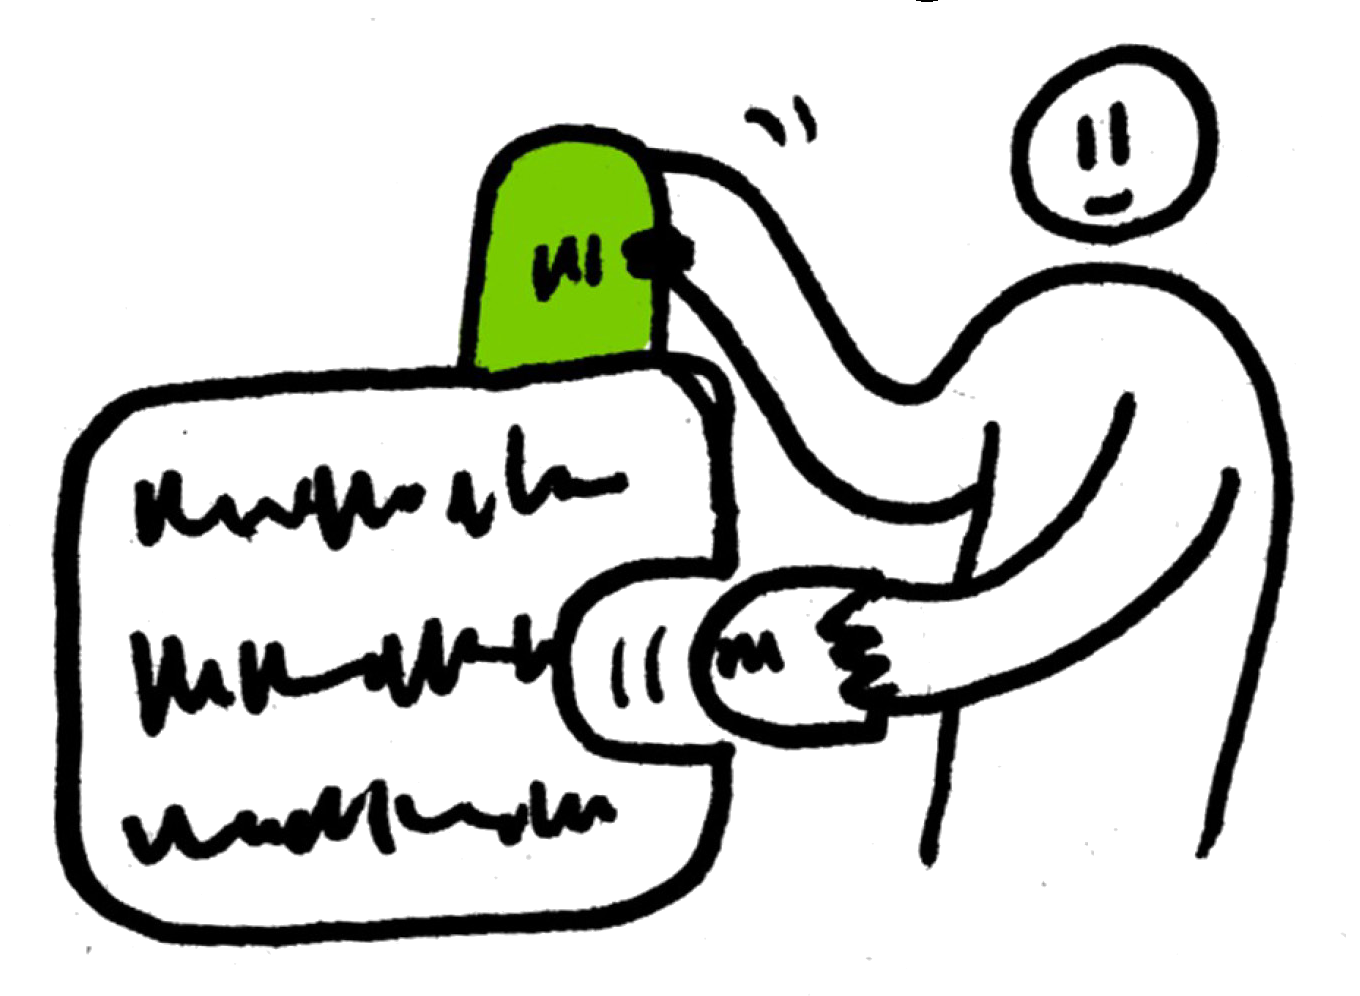
\includegraphics[scale=0.3]{fr-change}
    \caption{Freedom 1 : Mempelajari dan mengubah program}
  \end{figure}
\end{frame}

\begin{frame}
  \begin{figure}
    \frametitle{Apa itu Source Code}
    \centering
    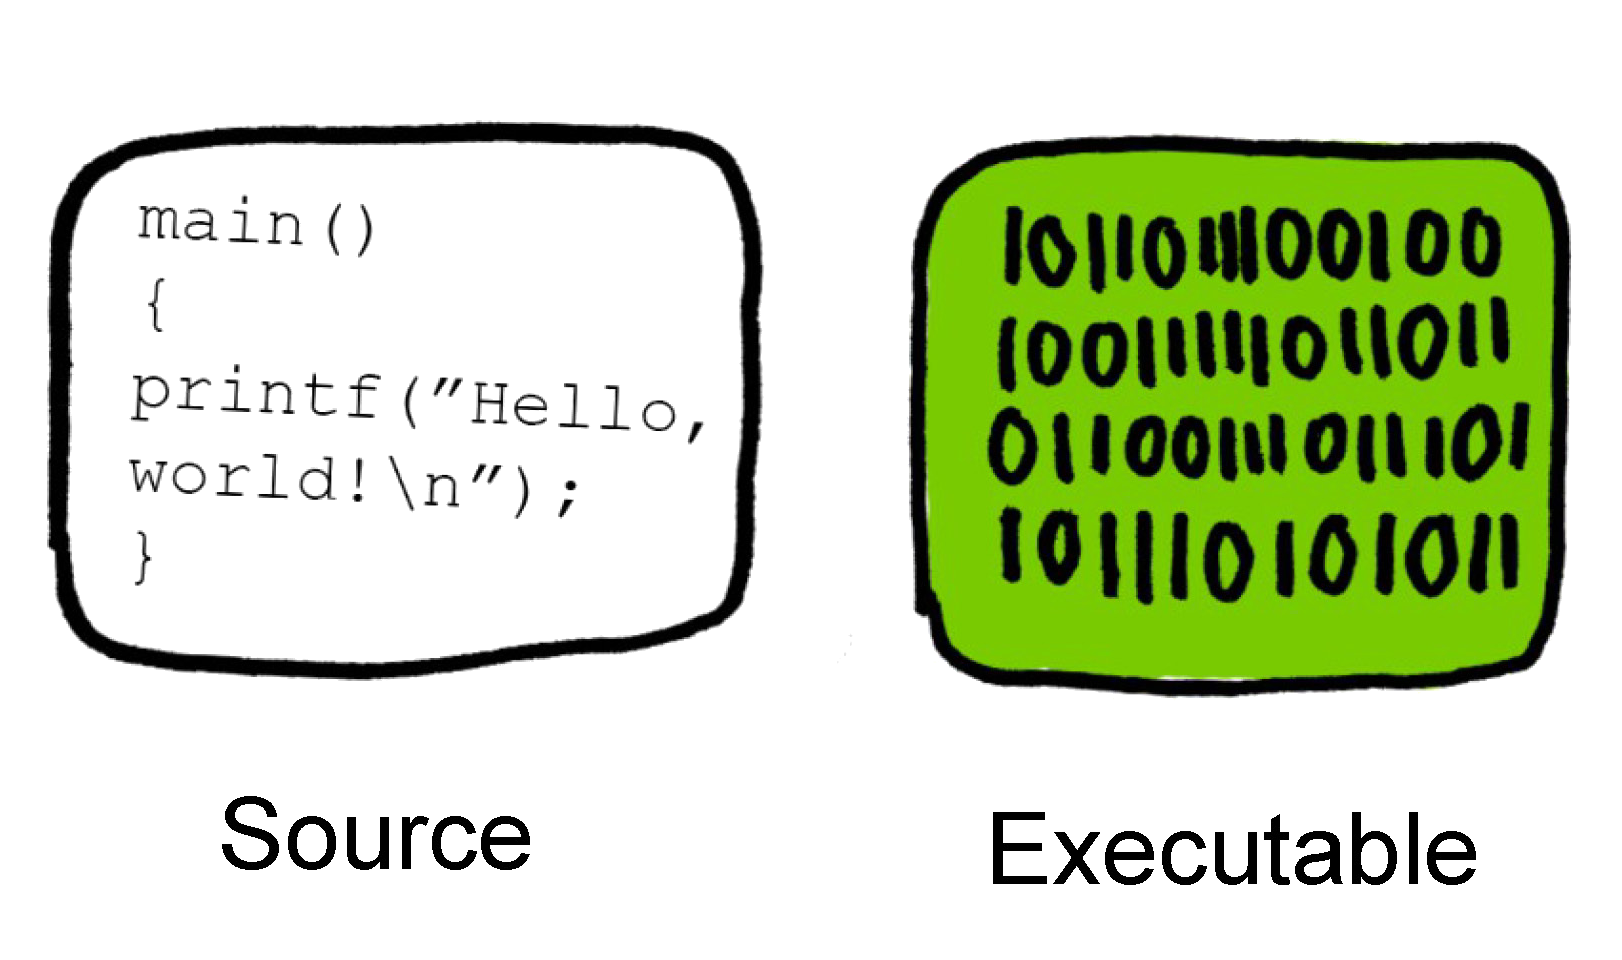
\includegraphics[scale=0.3]{source-code}
  \end{figure}
\end{frame}

\begin{frame}
  \begin{figure}
    % \frametitle{}
    \centering
    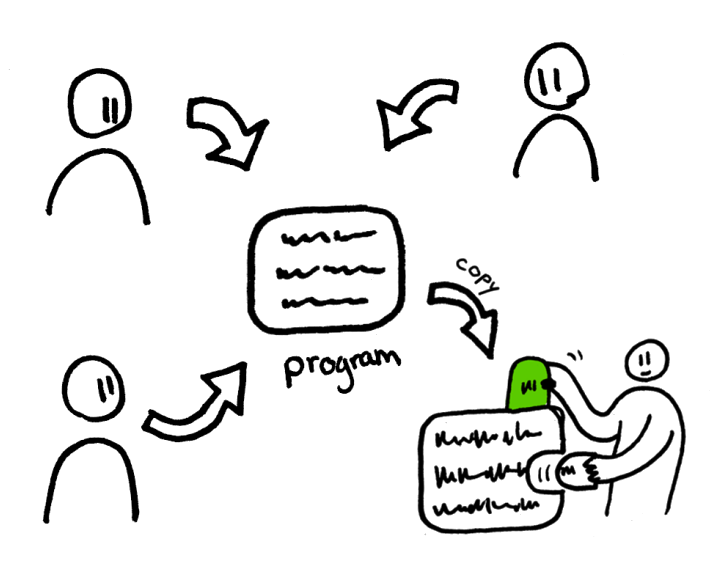
\includegraphics[scale=0.8]{make-copy}
    \caption{individual control}
  \end{figure}
\end{frame}

\begin{frame}
  \begin{figure}
    \frametitle{Bukan Programmer ?}
    \centering
    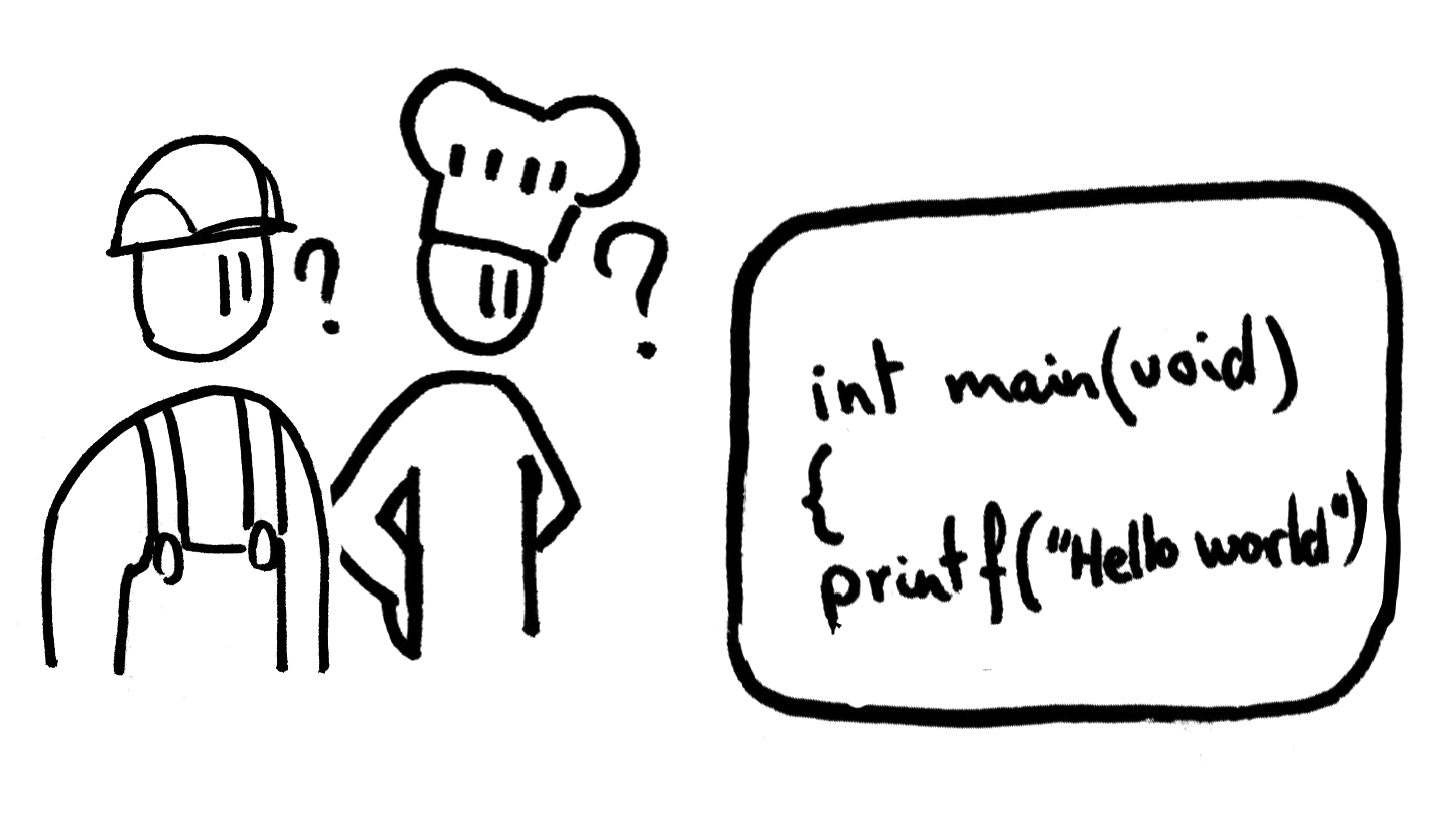
\includegraphics[scale=0.3]{not-programmer}
  \end{figure}
\end{frame}

\begin{frame}
  % \frametitle{}
  \begin{center}
    \Huge Kontrol individu tidak cukup
  \end{center}
\end{frame}

\begin{frame}
  \begin{figure}
    \frametitle{Collective Control}
    \centering
    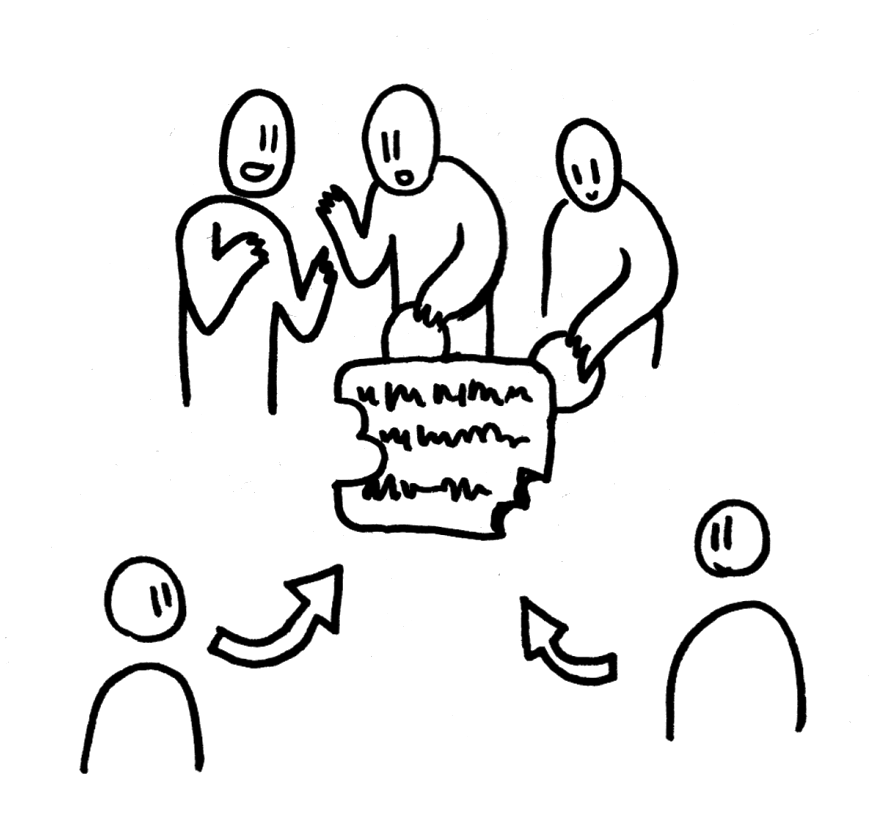
\includegraphics[scale=0.7]{collective-control}
  \end{figure}
\end{frame}

\begin{frame}
  \begin{figure}
    \frametitle{Kebebasan 2}
    \centering
    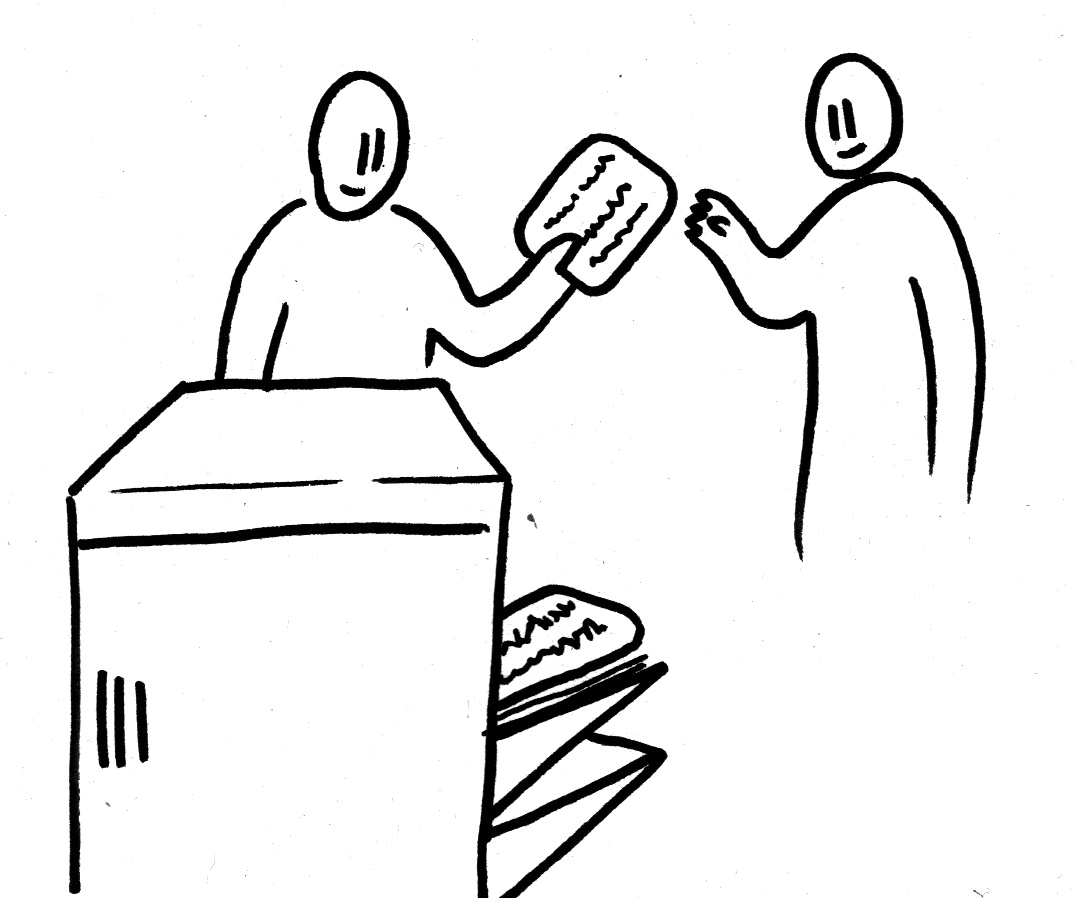
\includegraphics[scale=0.3]{fr-redistribute}
    \caption{Freedom 2 : Redistribusi}
  \end{figure}
\end{frame}

\begin{frame}
  \begin{figure}
    \frametitle{Kebebasan 3}
    \centering
    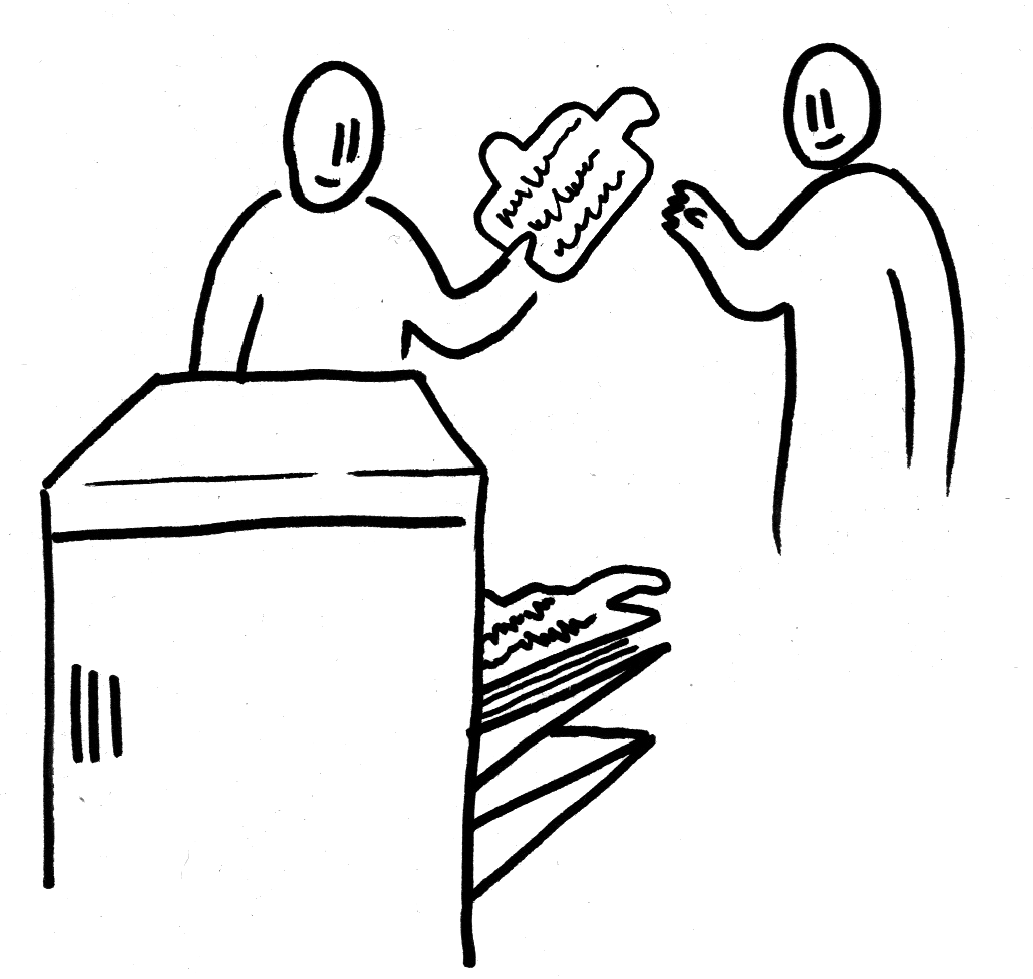
\includegraphics[scale=0.3]{fr-redistribute-chages}
    \caption{Freedom 3 : Redistribusi perubahan}    
  \end{figure}
\end{frame}


\begin{frame}
  \begin{figure}
    \frametitle{Pengguna mengatur program}
    \centering
    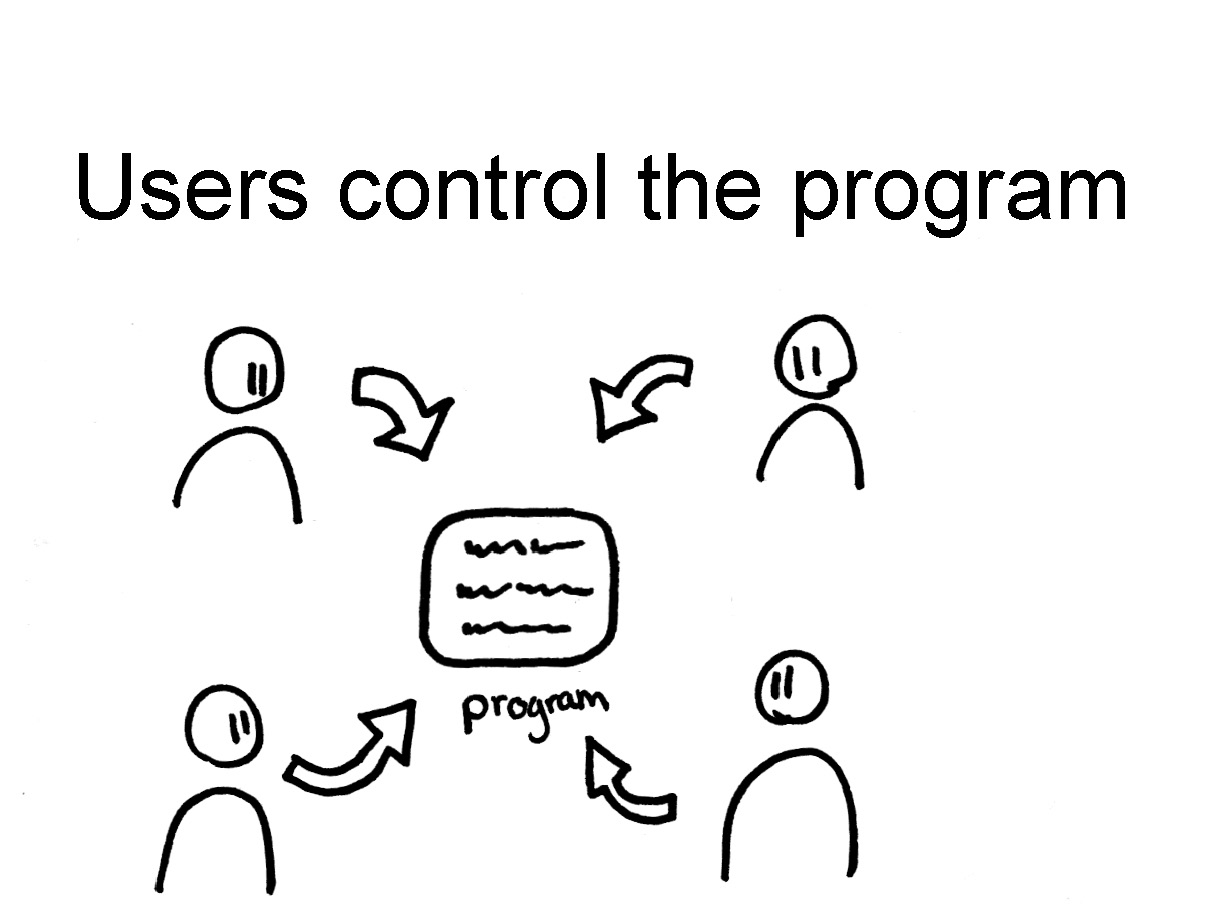
\includegraphics[scale=0.4]{user-control-program}
  \end{figure}
\end{frame}

\begin{frame}
  \begin{figure}
    \frametitle{Program mengatur user}
    \centering
    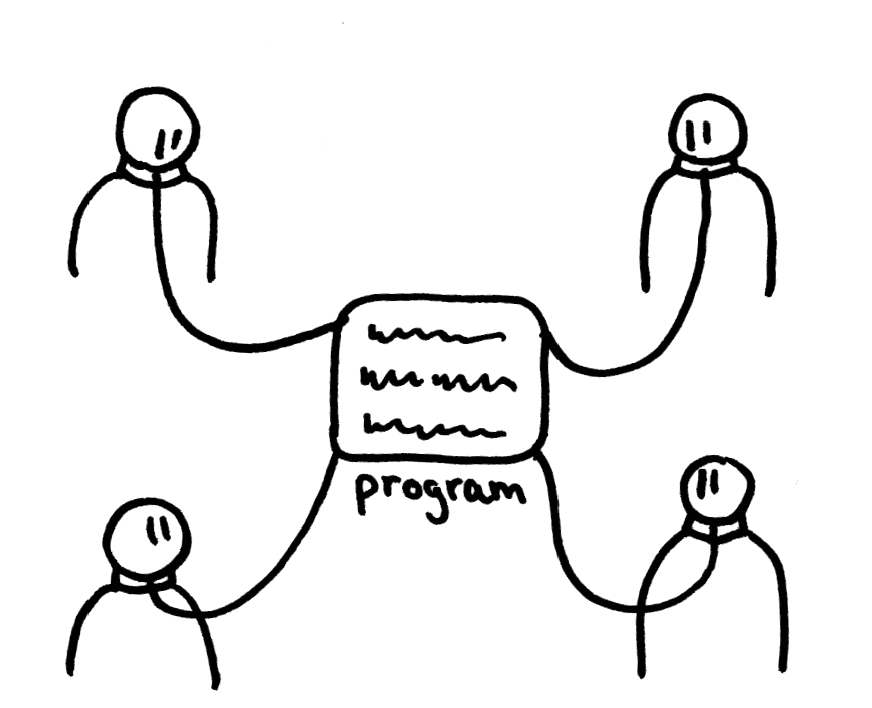
\includegraphics[scale=0.4]{program-control-user}
  \end{figure}
\end{frame}

\begin{frame}
  \begin{figure}
    \frametitle{Developer mengatur program}
    \centering
    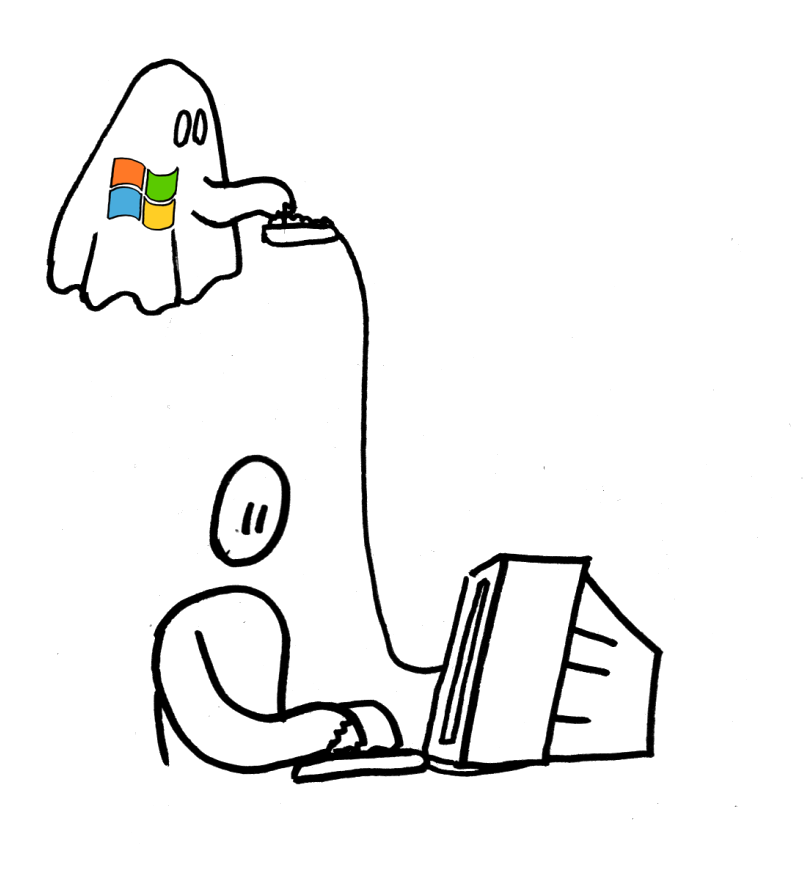
\includegraphics[scale=0.8]{ms-comp}
  \end{figure}
\end{frame}

\begin{frame}
  % \frametitle{}
  \begin{center}
    \Large Apa yang terjadi ketika kita menggunakan Proprietary Software ? \\
  \end{center}
\end{frame}

\begin{frame}
  \begin{figure}
    \centering
    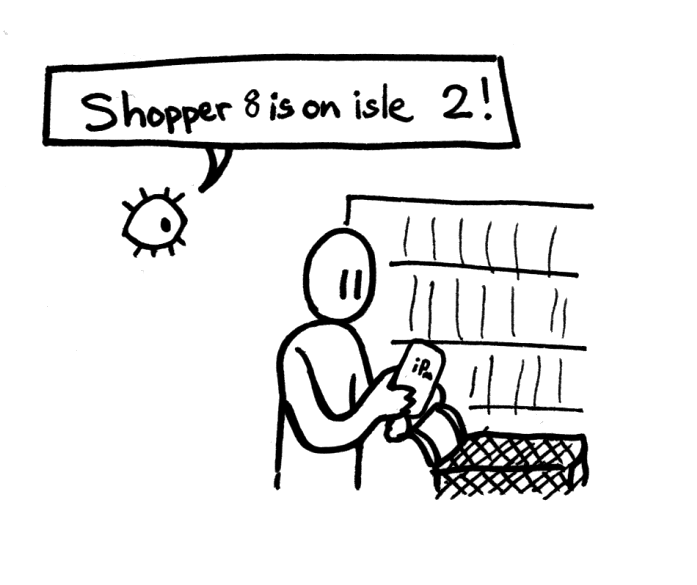
\includegraphics[scale=0.8]{pr-track}
  \end{figure}
\end{frame}

\begin{frame}
  \begin{figure}
    \centering
    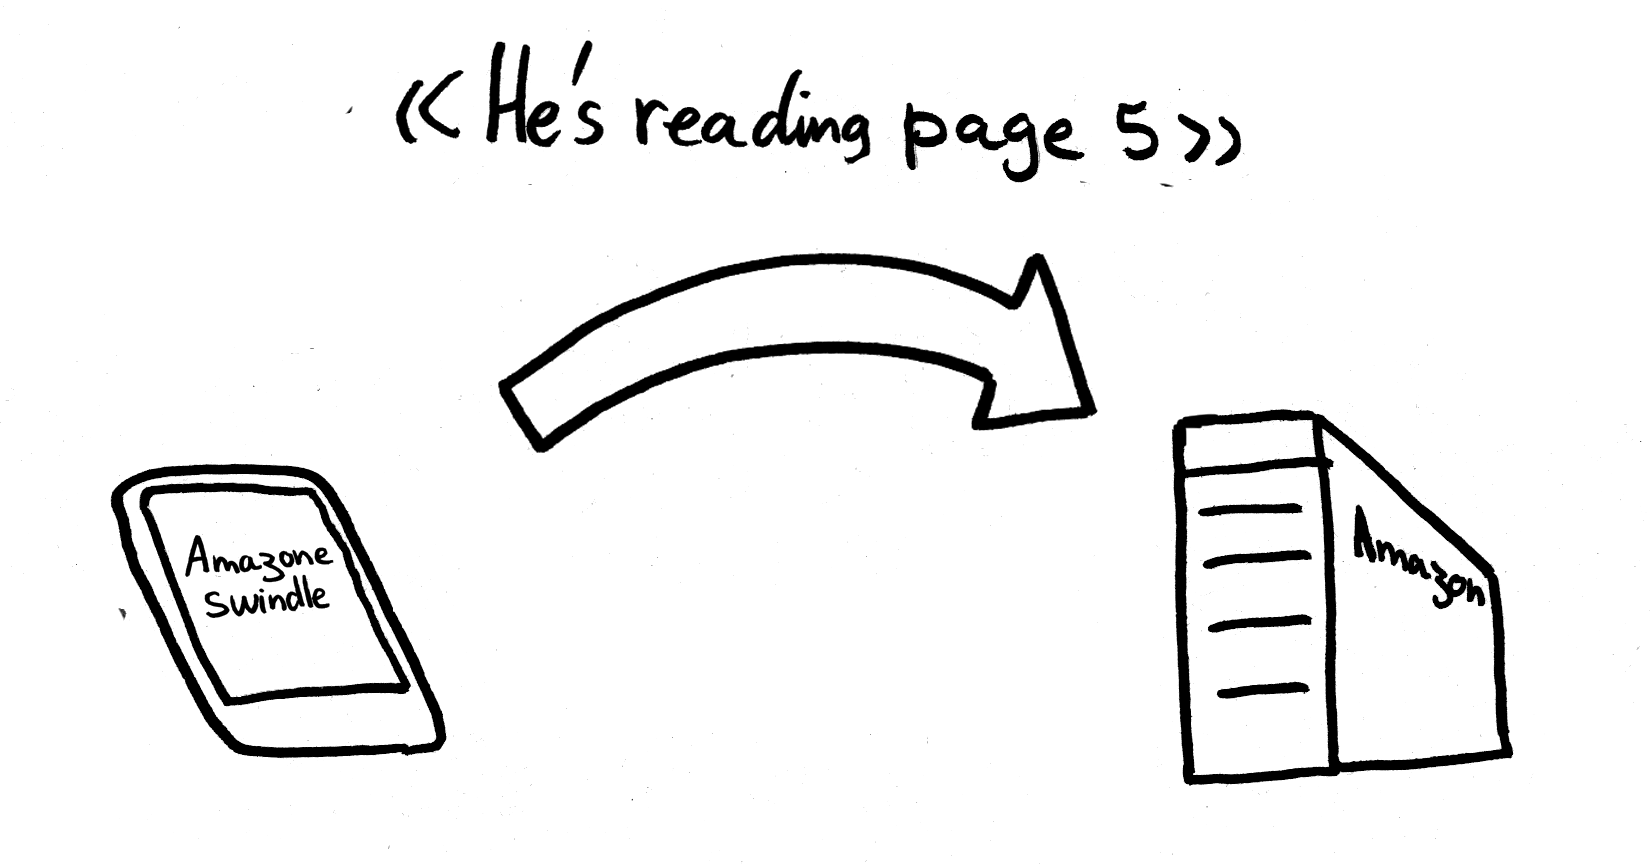
\includegraphics[scale=0.8]{pr-snoops}
  \end{figure}
\end{frame}

\begin{frame}
  \begin{figure}
    \centering
    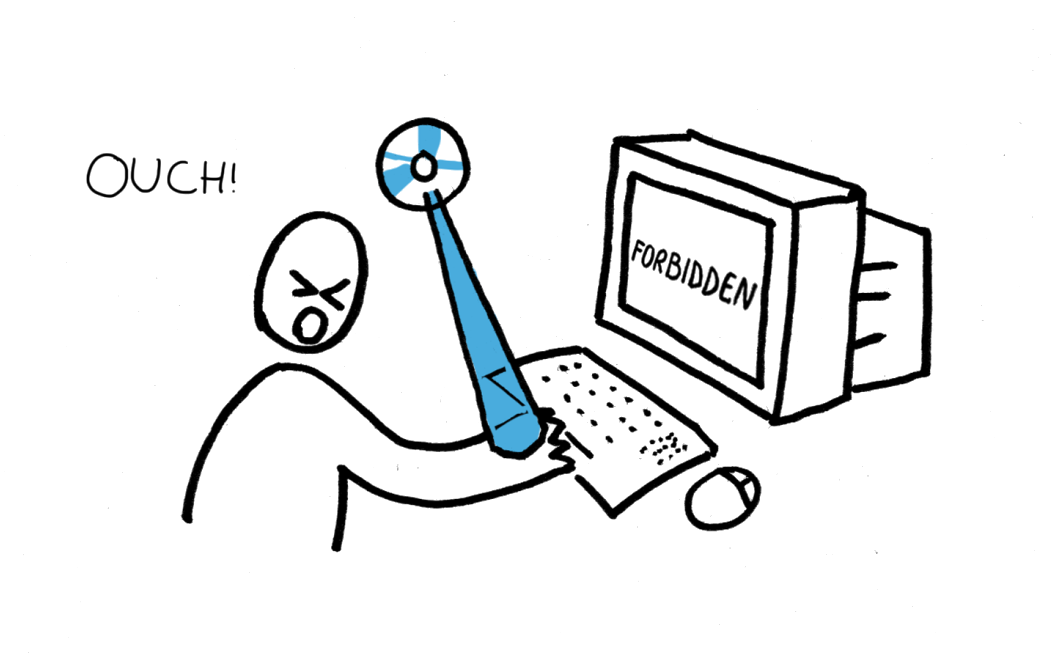
\includegraphics[scale=0.8]{pr-restrict}
  \end{figure}
\end{frame}

\begin{frame}
  \begin{figure}
    \centering
    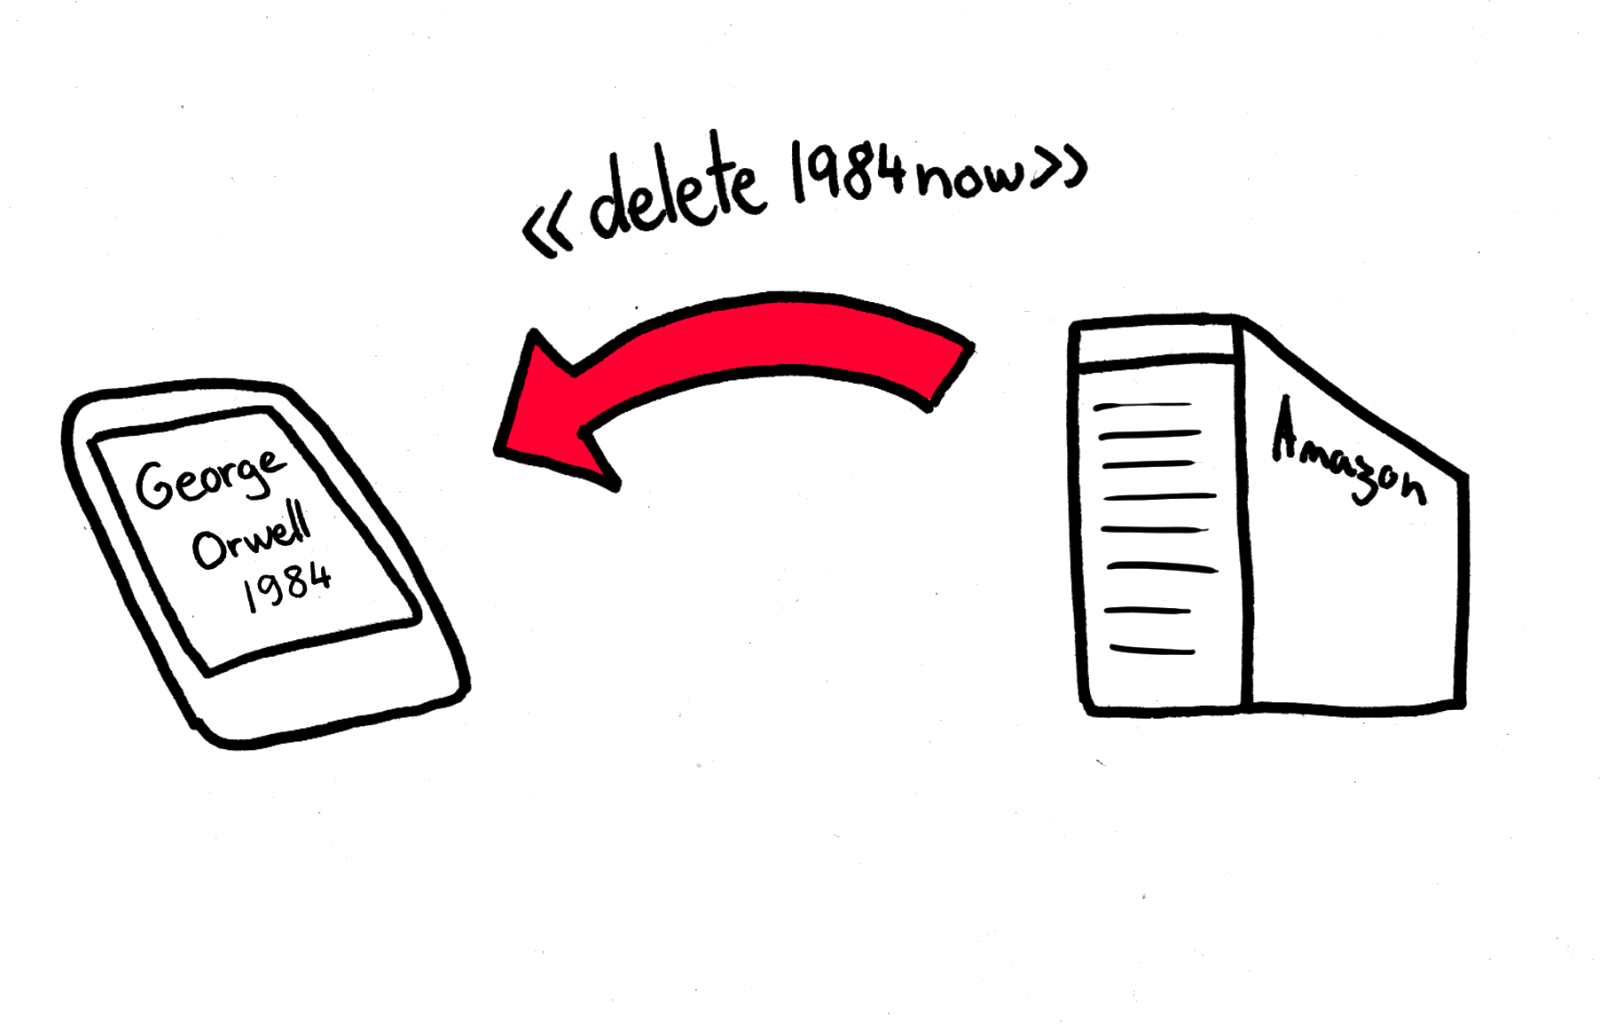
\includegraphics[scale=0.5]{pr-remote-delete}
  \end{figure}
\end{frame}

\begin{frame}
  \begin{figure}
    \centering
    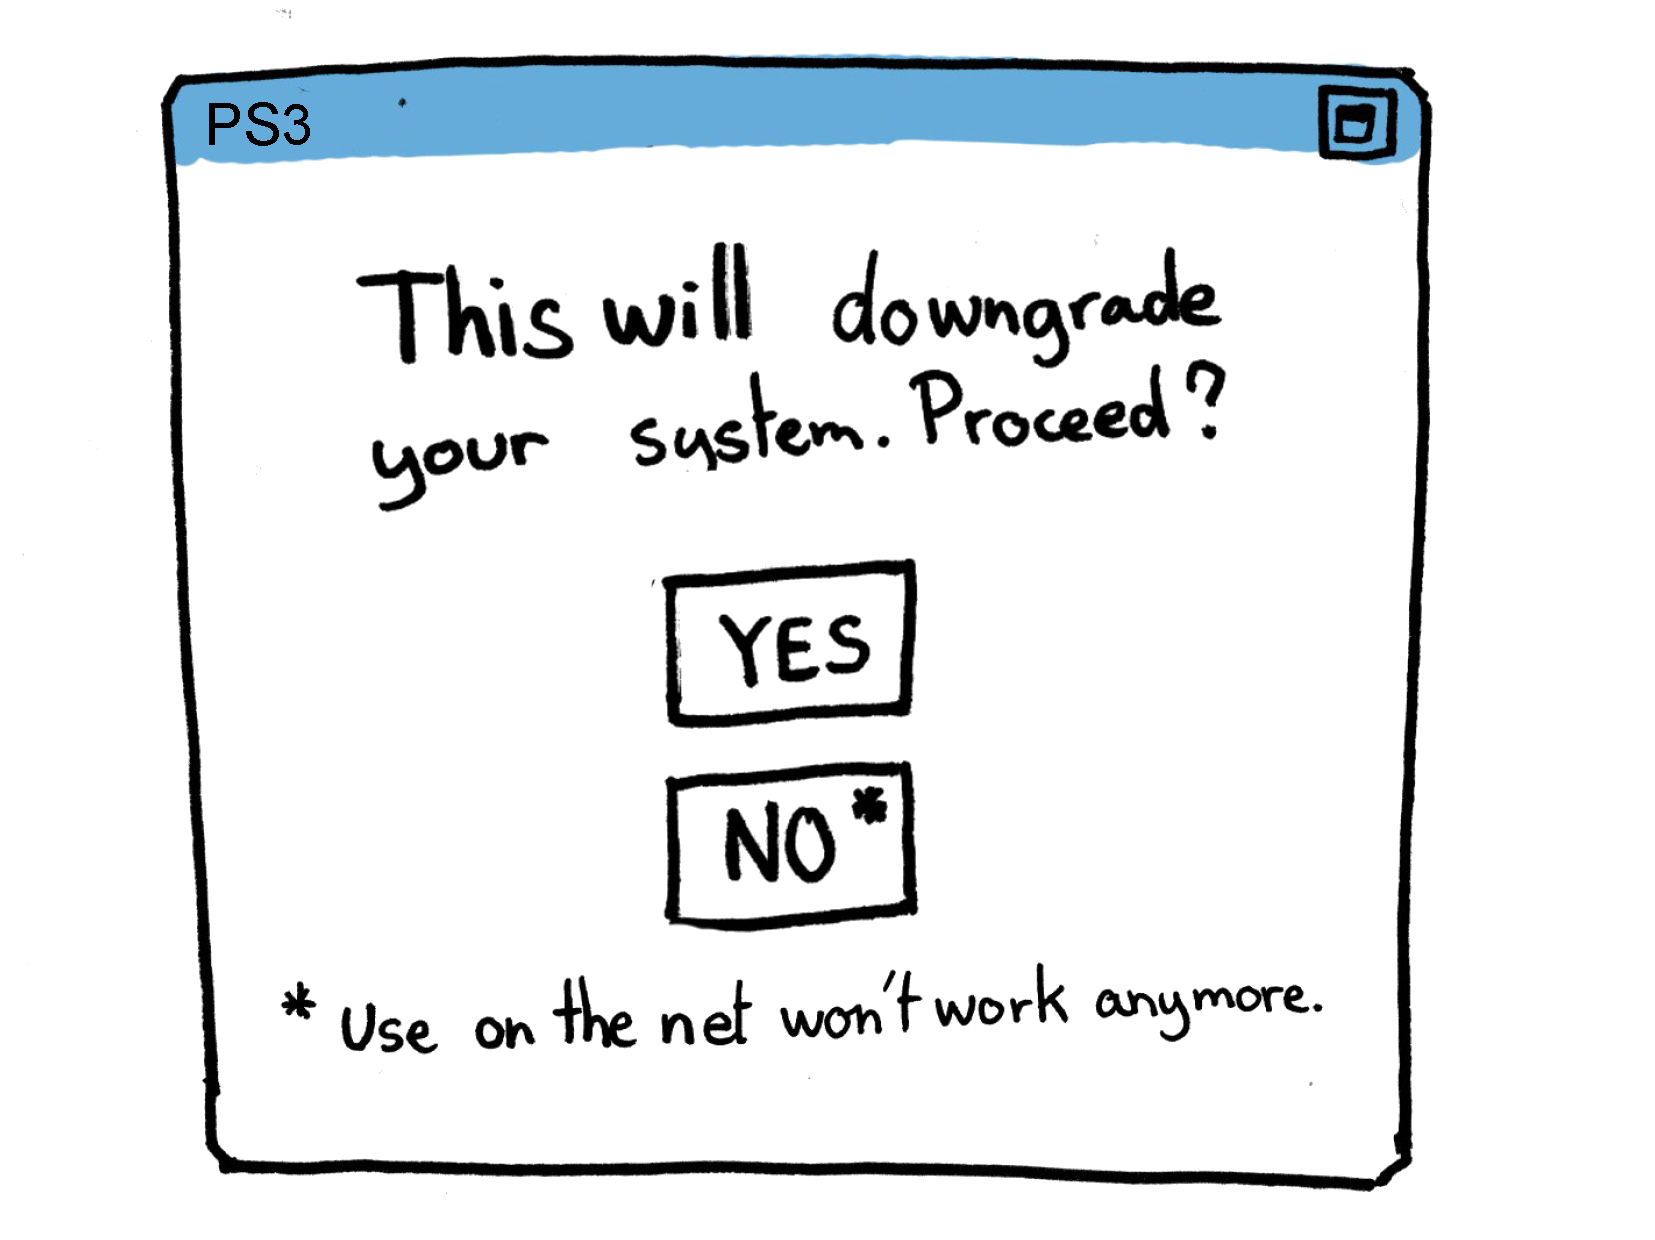
\includegraphics[scale=0.4]{pr-compels}
  \end{figure}
\end{frame}

\begin{frame}
  \begin{figure}
    \centering
    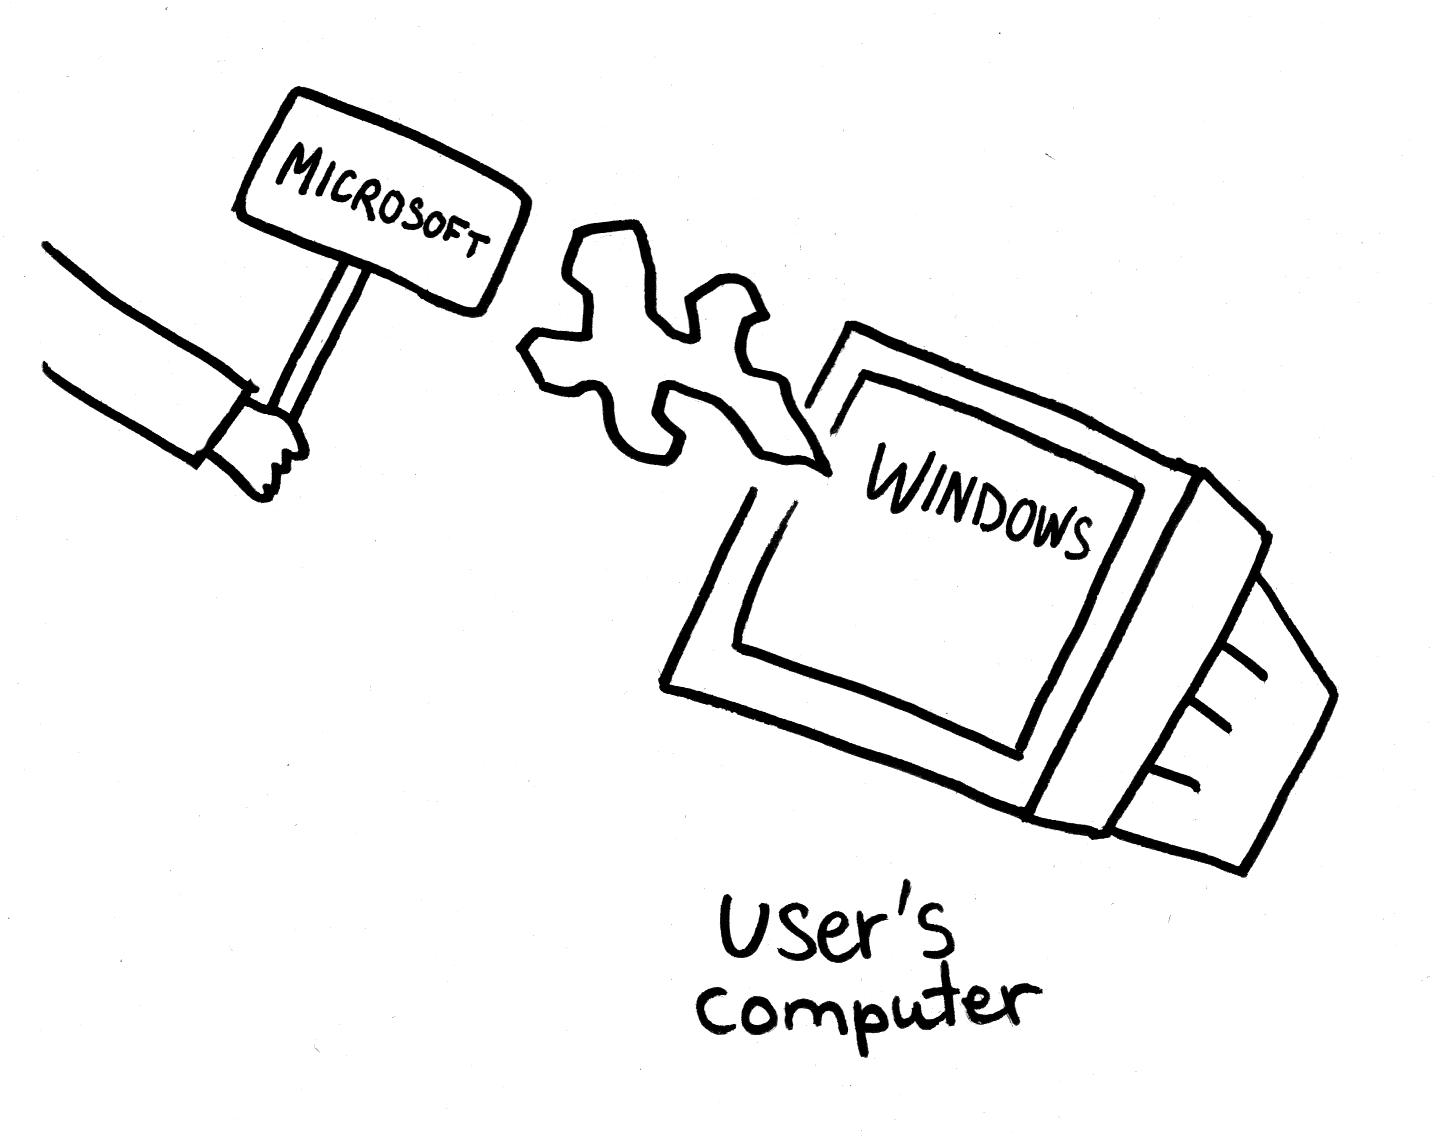
\includegraphics[scale=0.8]{pr-remote-changes}
  \end{figure}
\end{frame}


\begin{frame}
  \begin{figure}
    \centering
    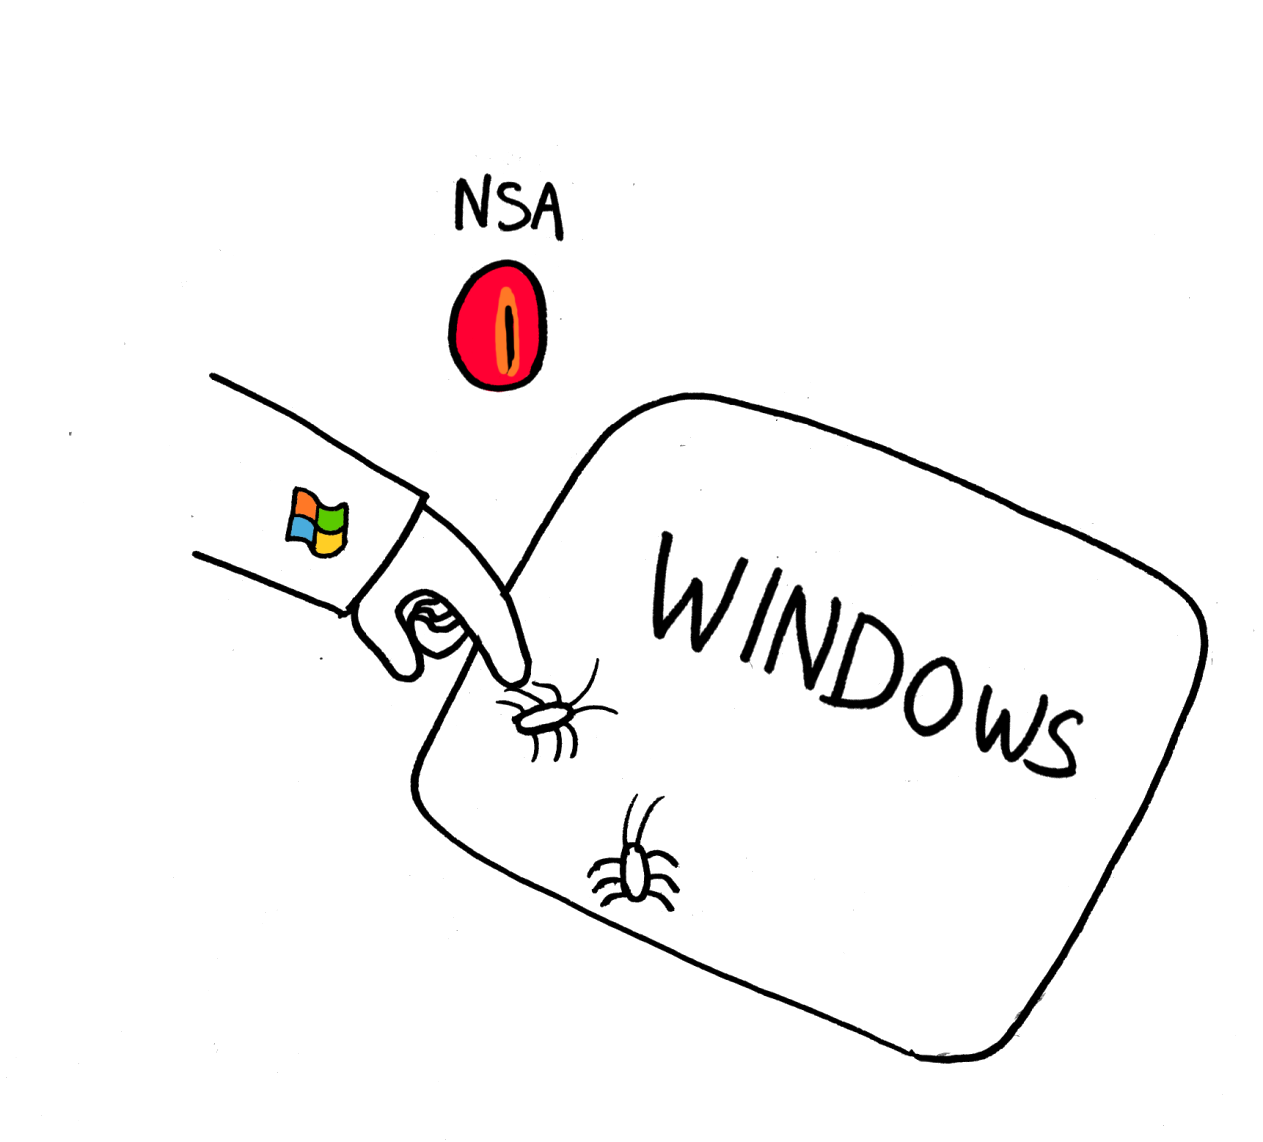
\includegraphics[scale=0.6]{pr-tell-nsa}
  \end{figure}
\end{frame}

\begin{frame}
  \begin{figure}
    \centering
    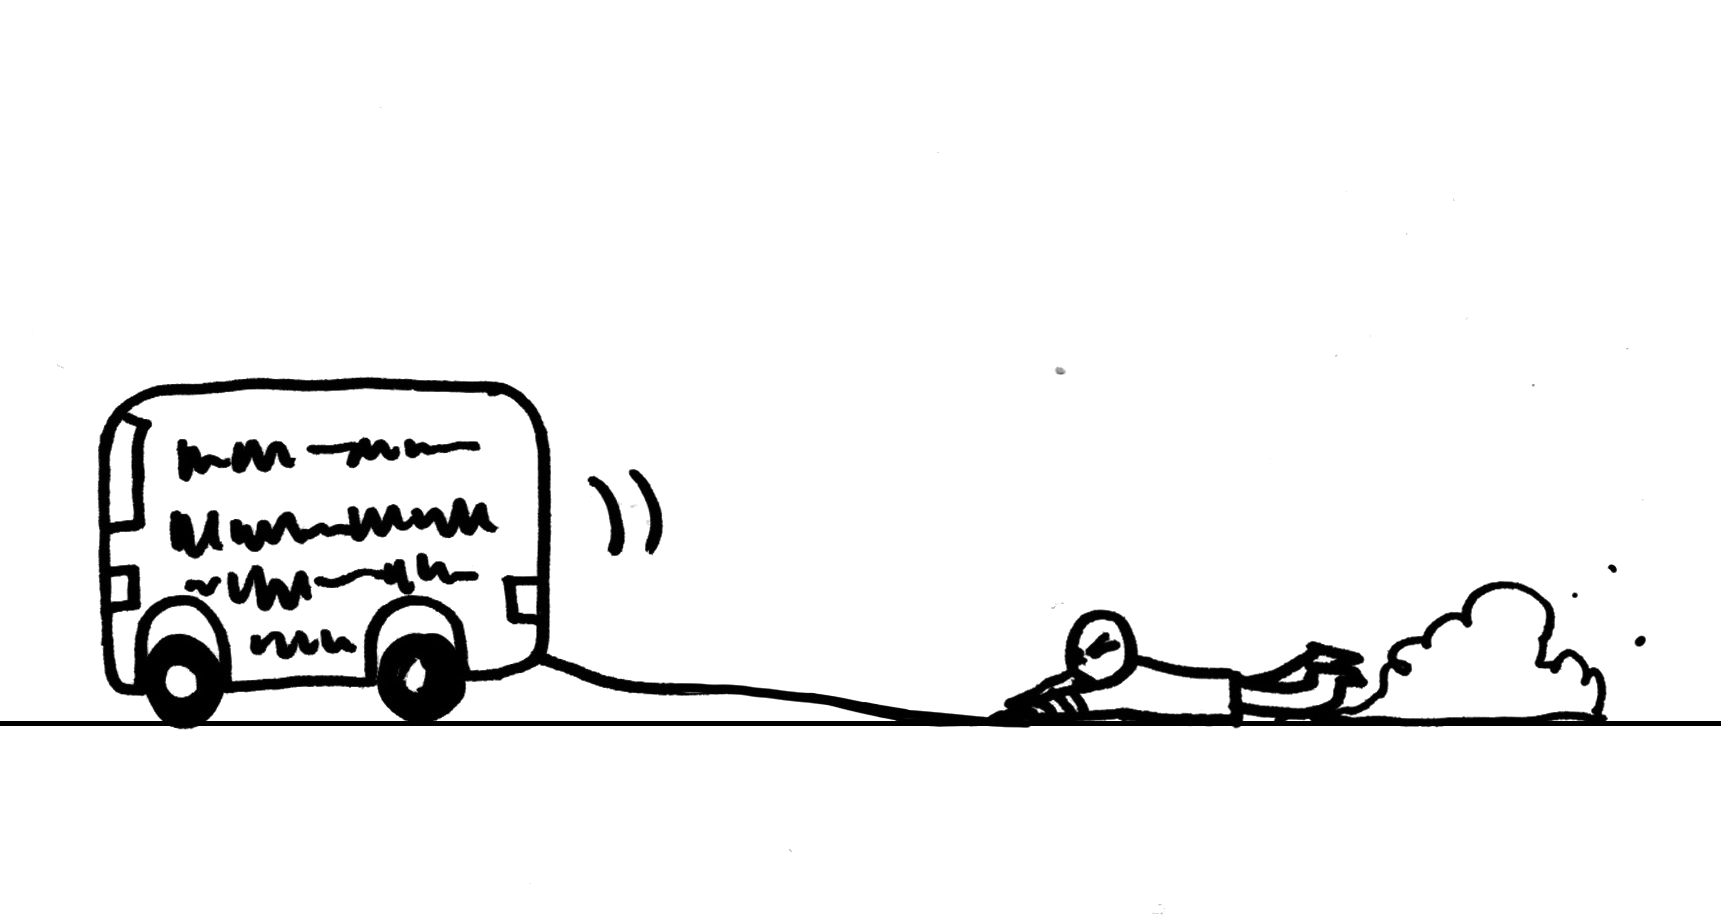
\includegraphics[scale=0.5]{pr-injury}
  \end{figure}
\end{frame}

\begin{frame}
  \begin{figure}
    \centering
    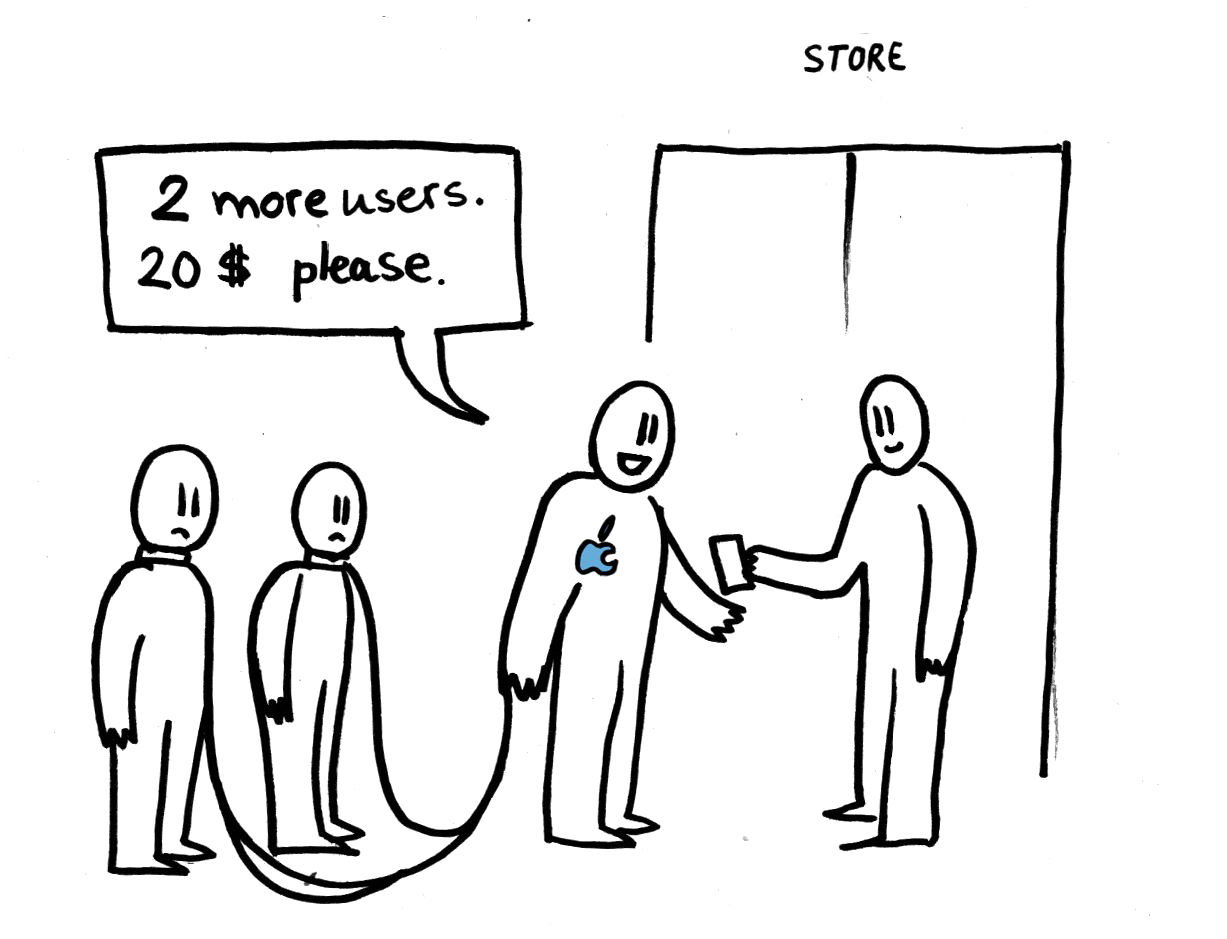
\includegraphics[scale=0.4]{pr-sake-of-money}
  \end{figure}
\end{frame}

\begin{frame}
  \begin{figure}
    \centering
    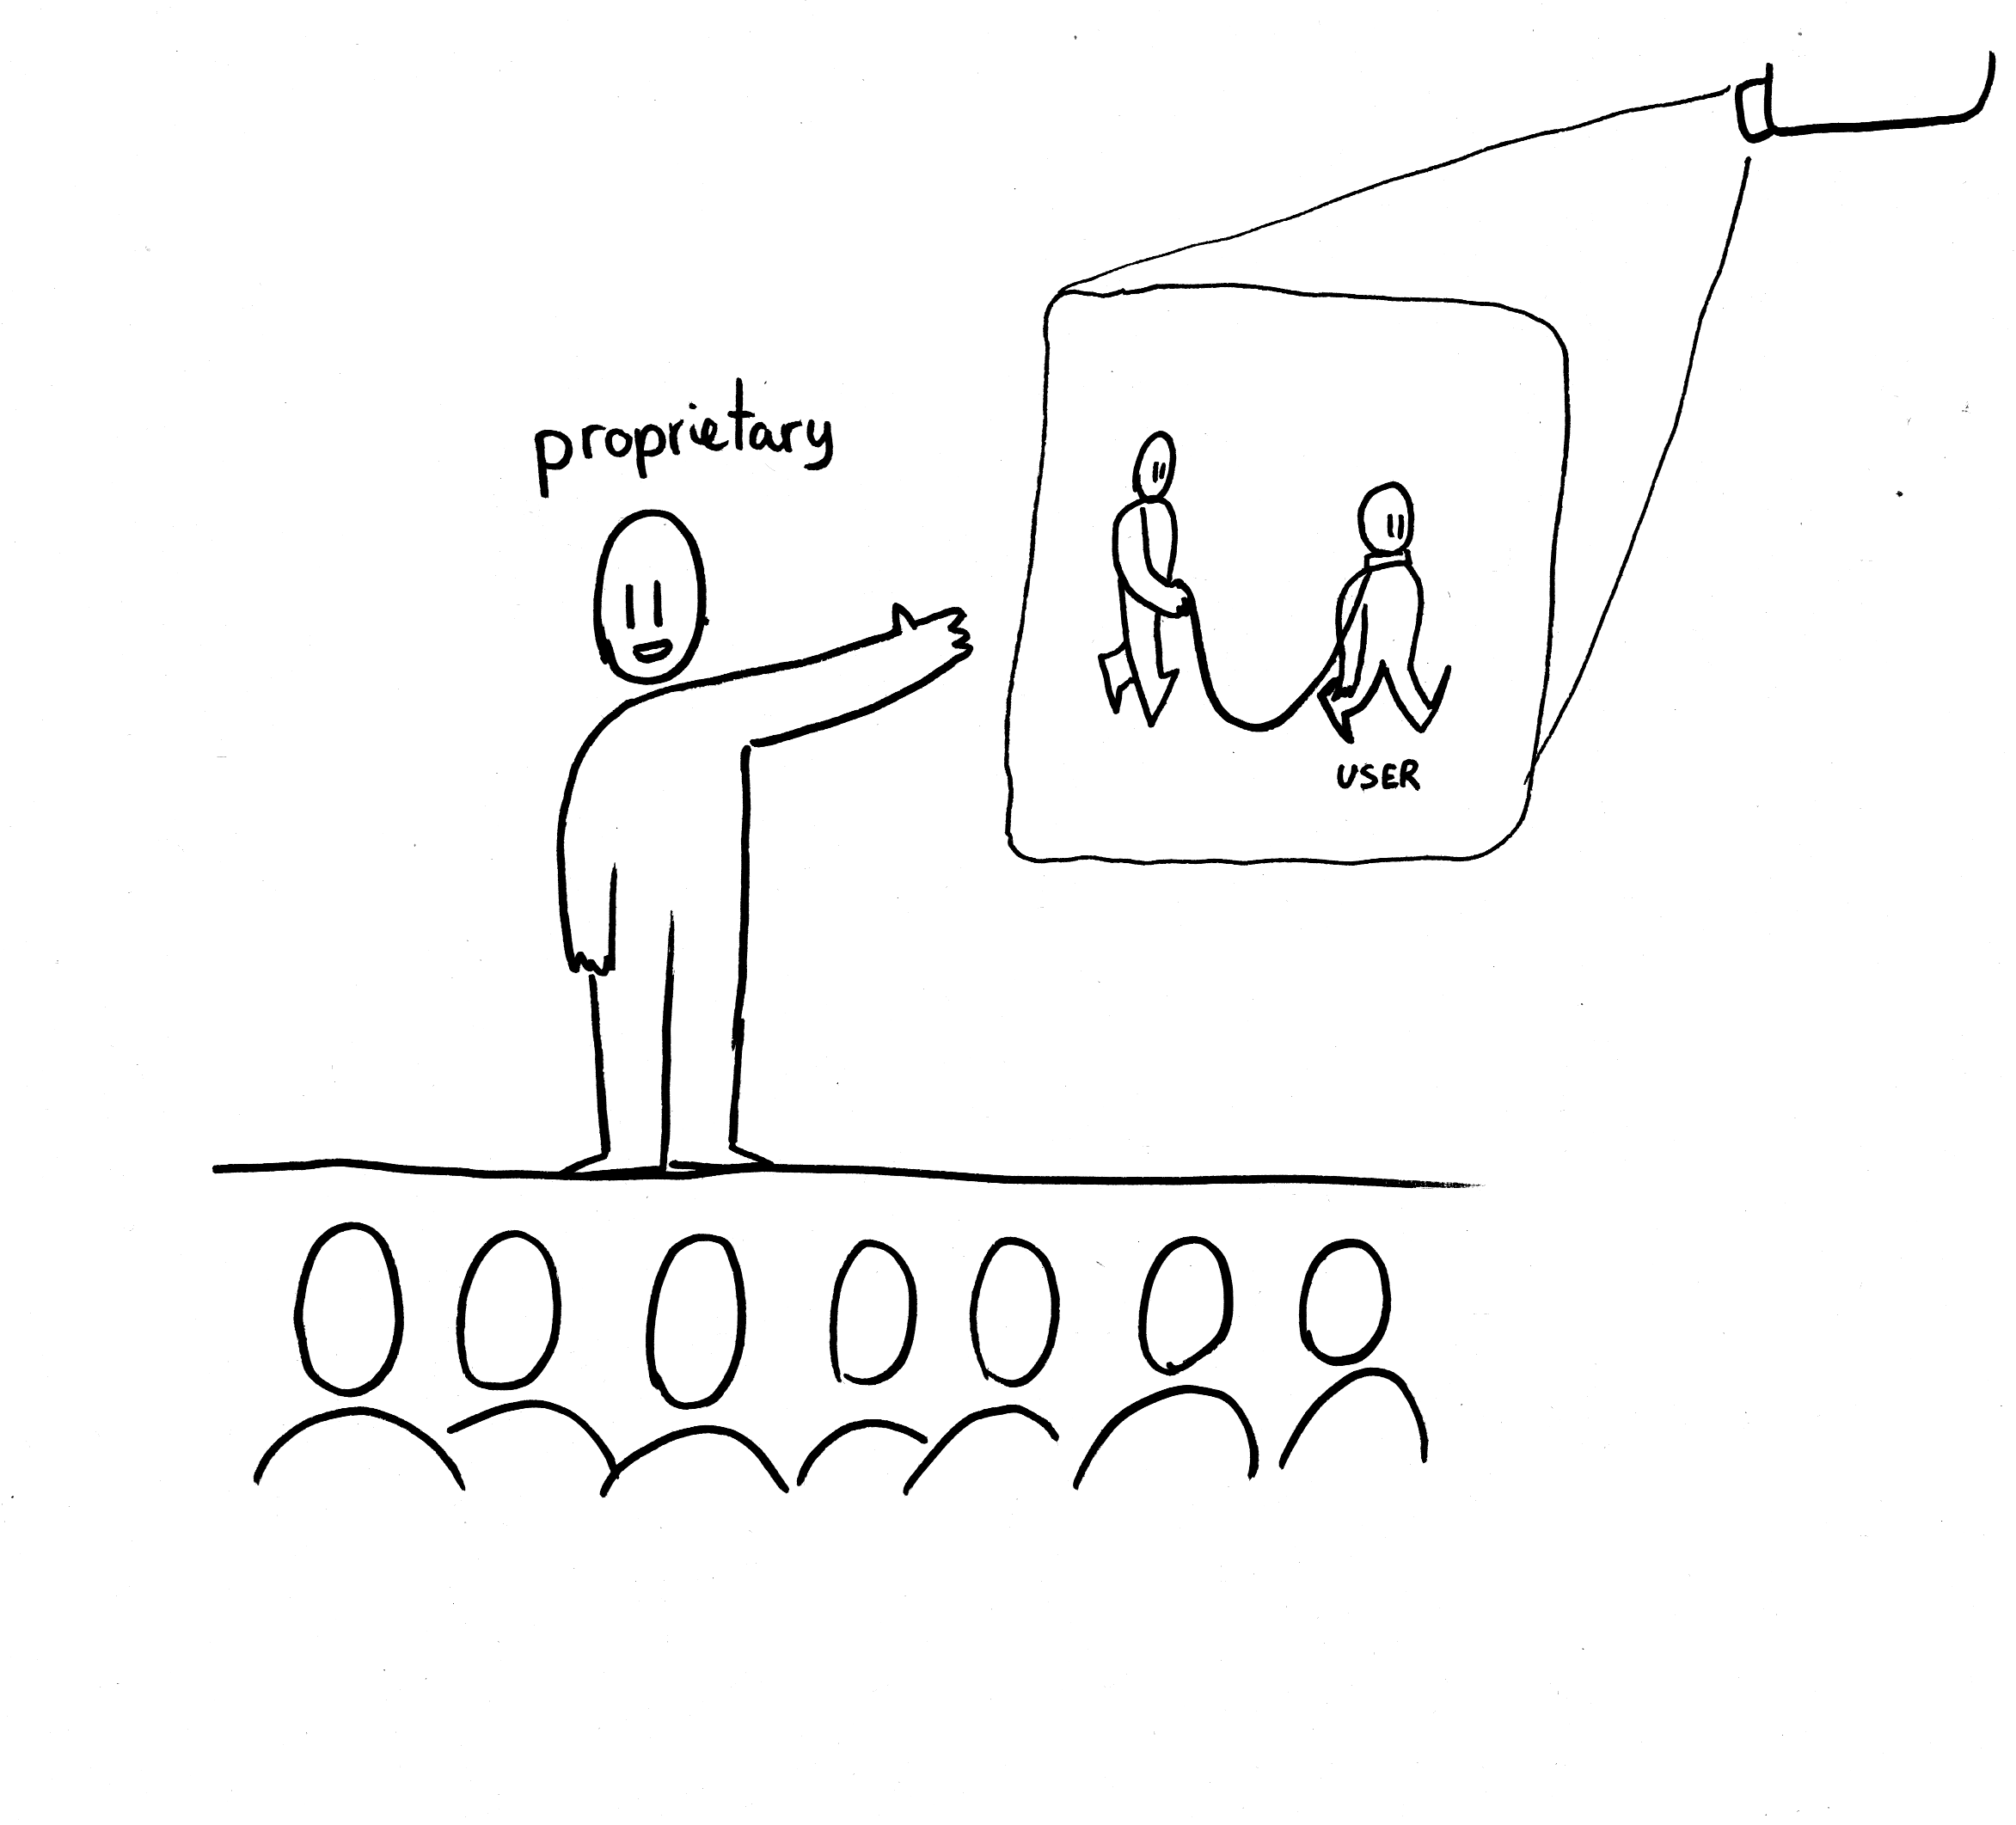
\includegraphics[scale=0.5]{pr-no-shame}
  \end{figure}
\end{frame}

\begin{frame}
  % \frametitle{}
  \begin{center}
    \Huge Jadi, bagaimana agar kita tidak menjadi korban ?
  \end{center}
\end{frame}

\begin{frame}
  \color{red}
  % \frametitle{}
  \begin{center}
    \Huge Berhenti menggunakan \textit{Computer}.
  \end{center}
\end{frame}

\begin{frame}
  \begin{figure}
    \centering
    \large Selamat Datang, bergabunglah.
    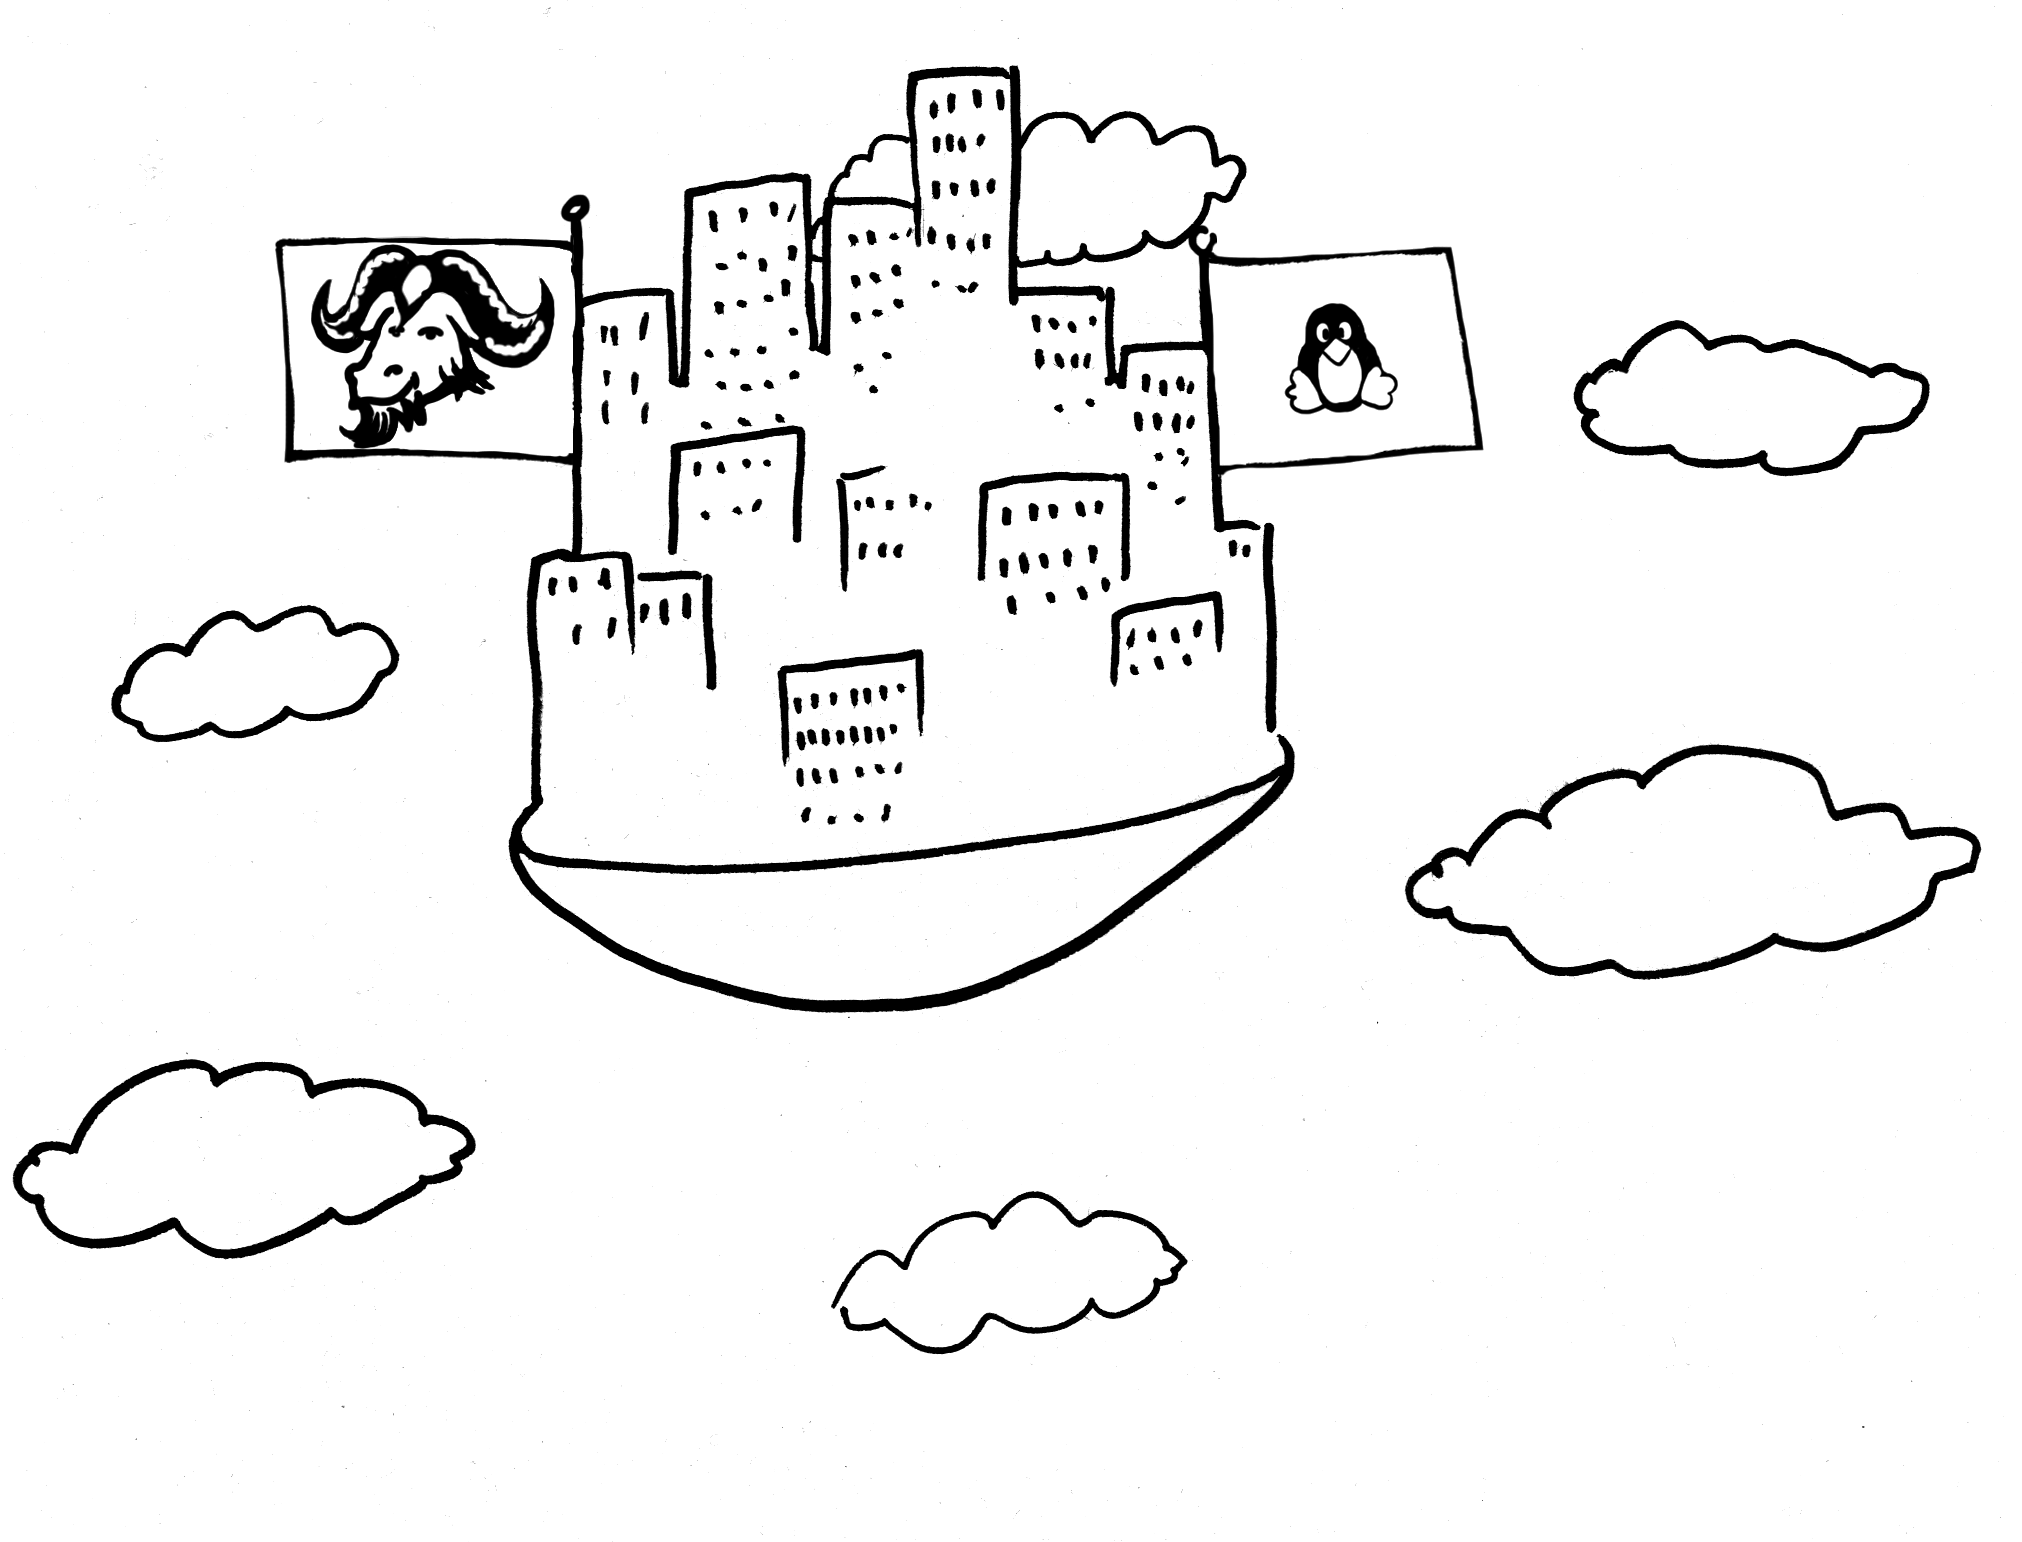
\includegraphics[scale=0.5]{gnu-linux-world}
  \end{figure}
\end{frame}

\begin{frame}
  \begin{figure}
    \centering
    \large Pengorbanan besar untuk kebebasan
    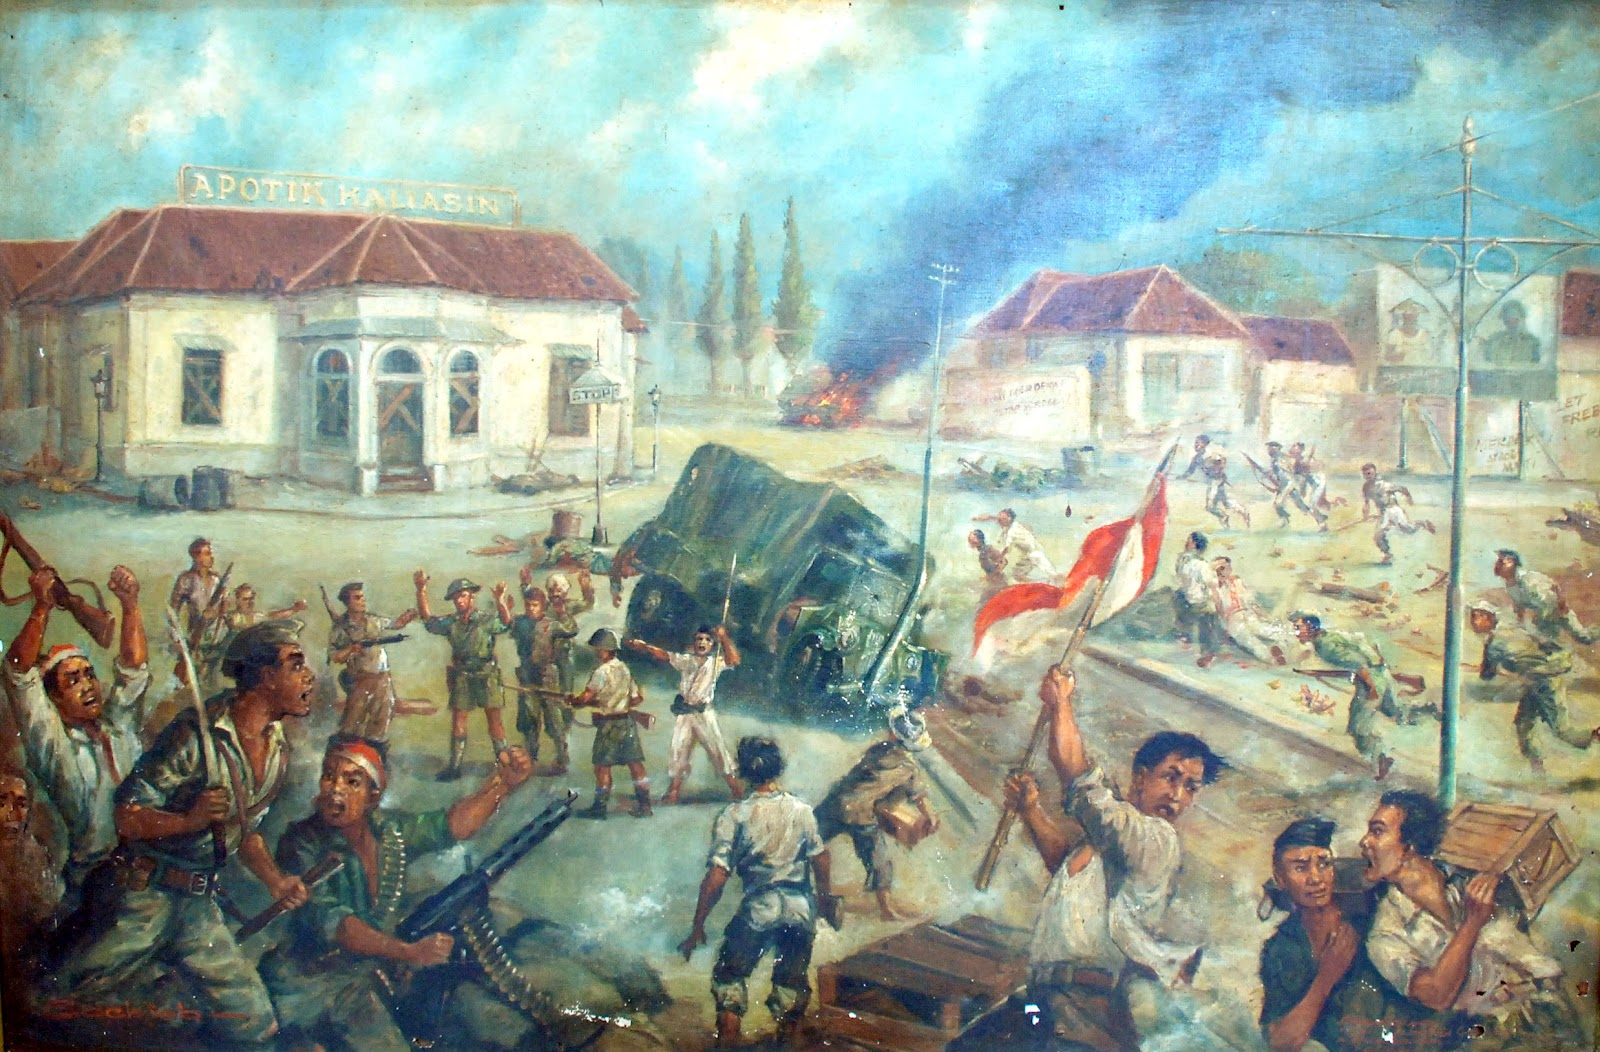
\includegraphics[scale=0.1]{ind-war}
  \end{figure}
\end{frame}

\begin{frame}
  \begin{figure}
    \centering
    \large Pengorbanan kecil untuk kebebasan
    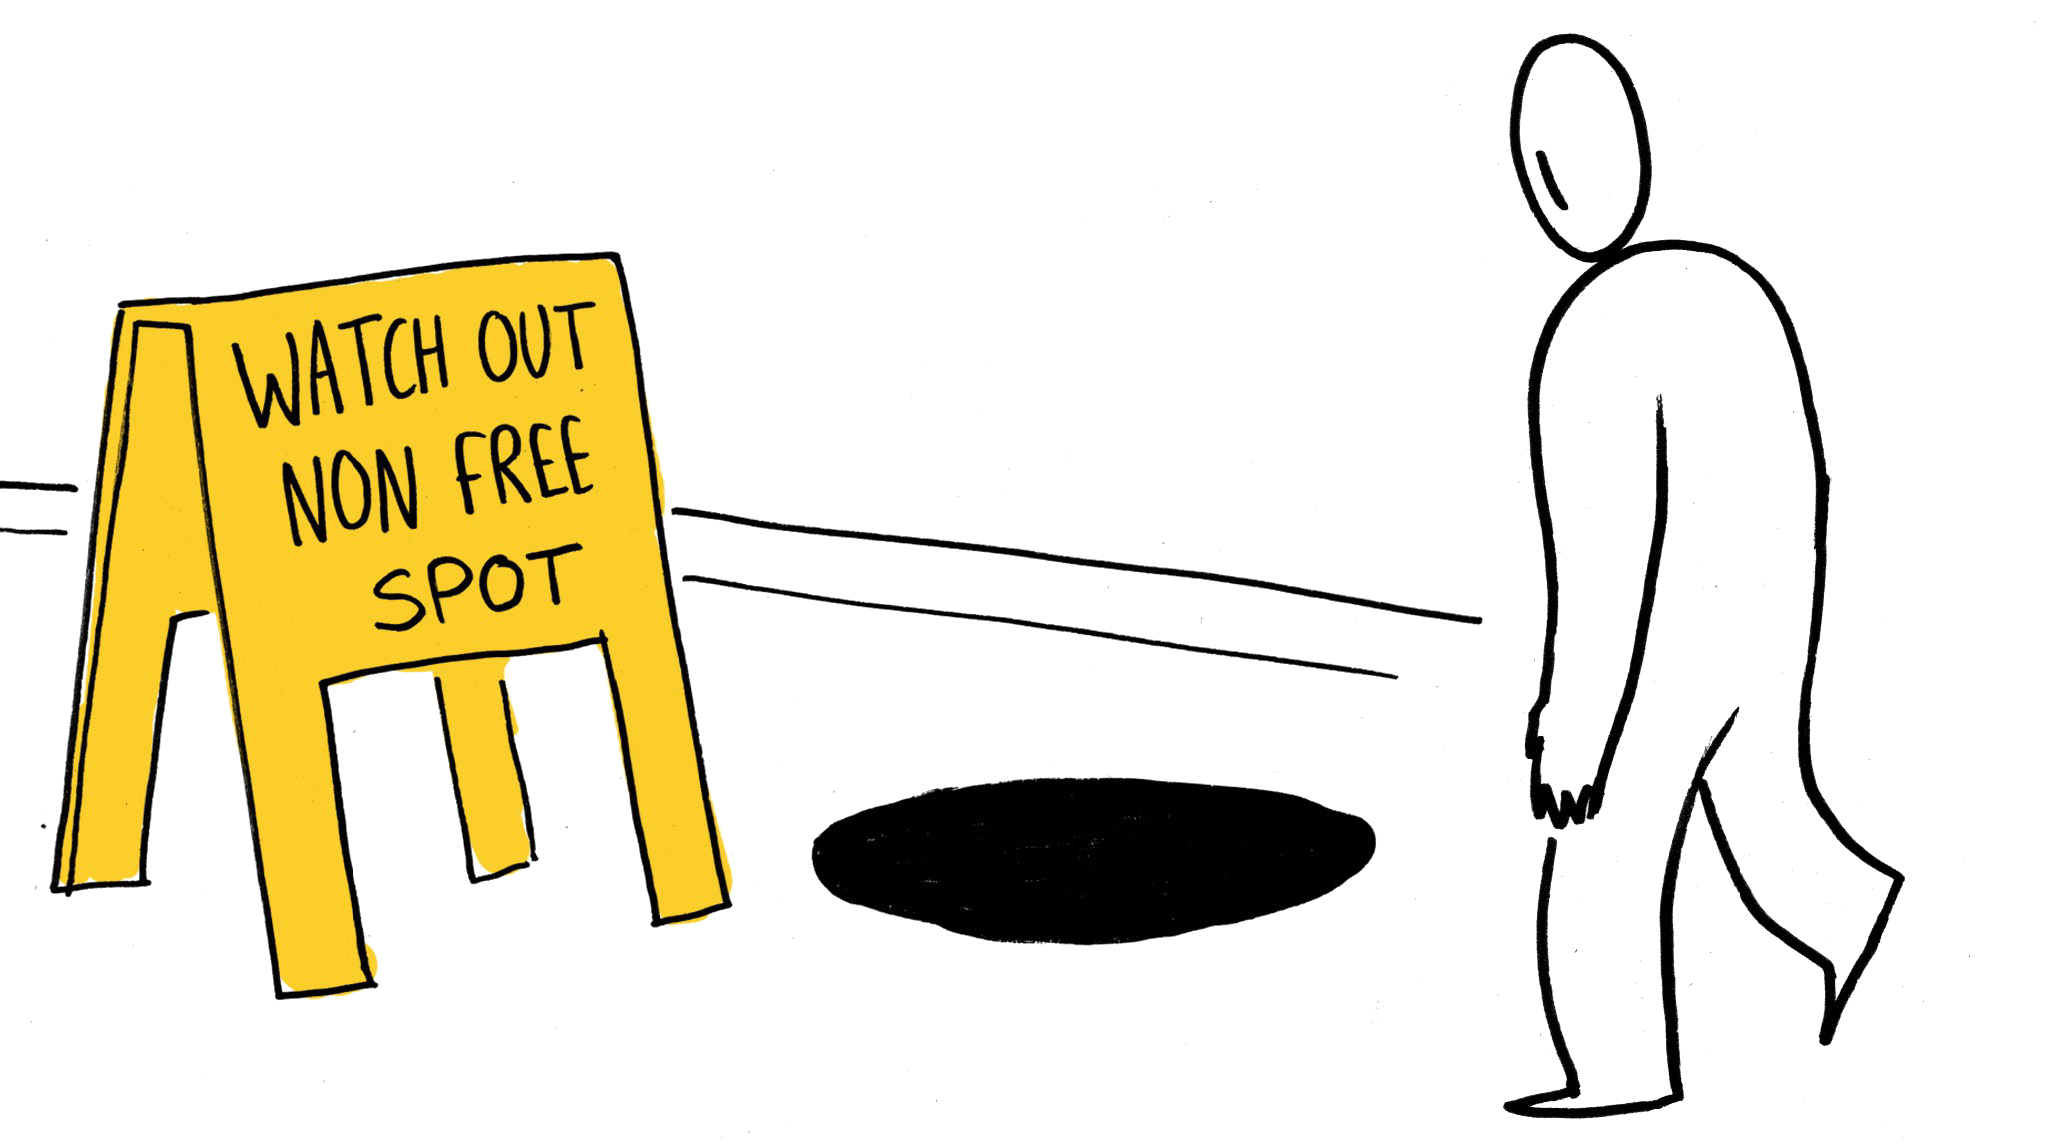
\includegraphics[scale=0.5]{fs-small-sacrifice}
  \end{figure}
\end{frame}

\begin{frame}
  \begin{figure}
    \centering
    
\includegraphics[scale=0.5]{non-free-at-gnu}
  \end{figure}
\end{frame}

\begin{frame}
  \begin{figure}
    \centering
    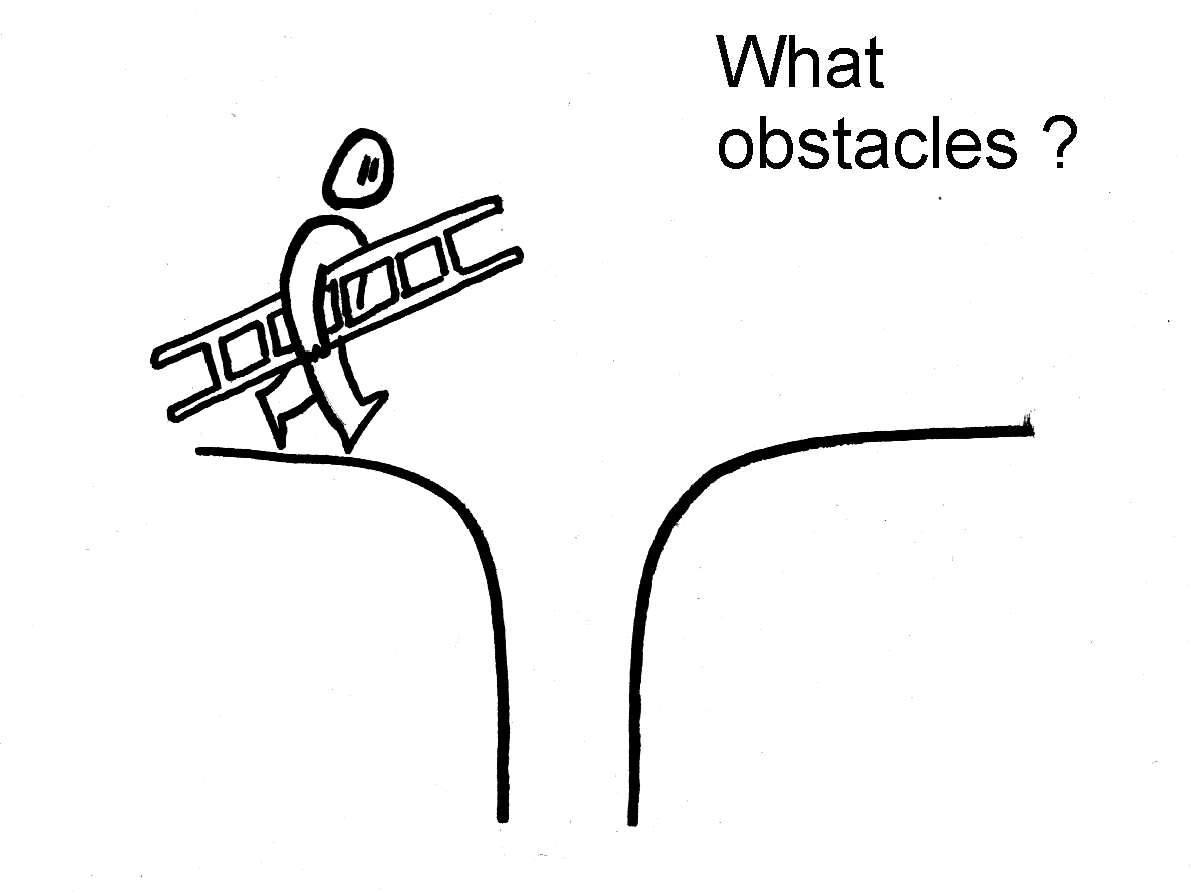
\includegraphics[scale=0.3]{cross-obstacles}
  \end{figure}
\end{frame}

\begin{frame}
  \begin{figure}
    \centering
    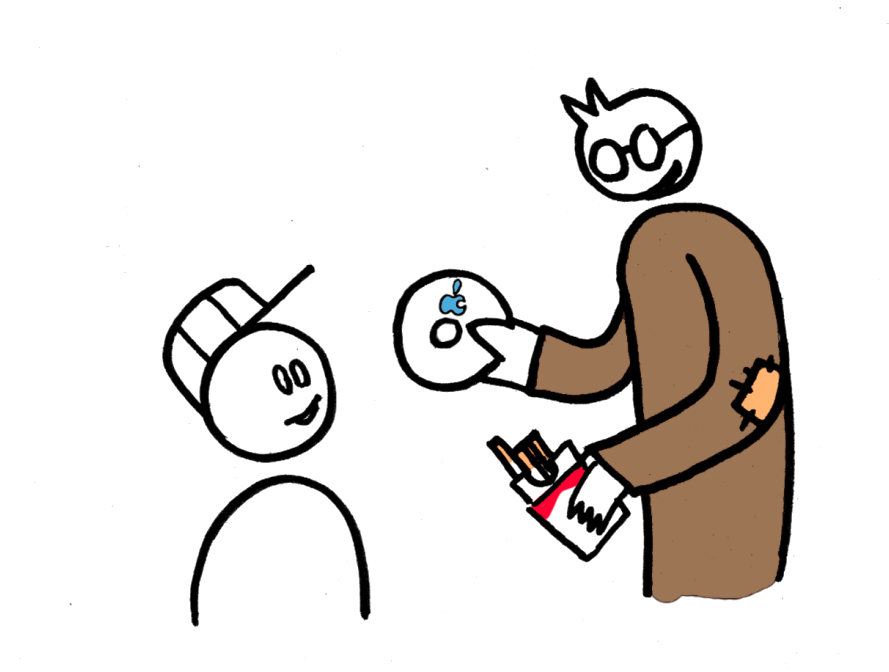
\includegraphics[scale=0.8]{teach-tobacco}
  \end{figure}
\end{frame}

\begin{frame}
  \begin{figure}
    \centering
    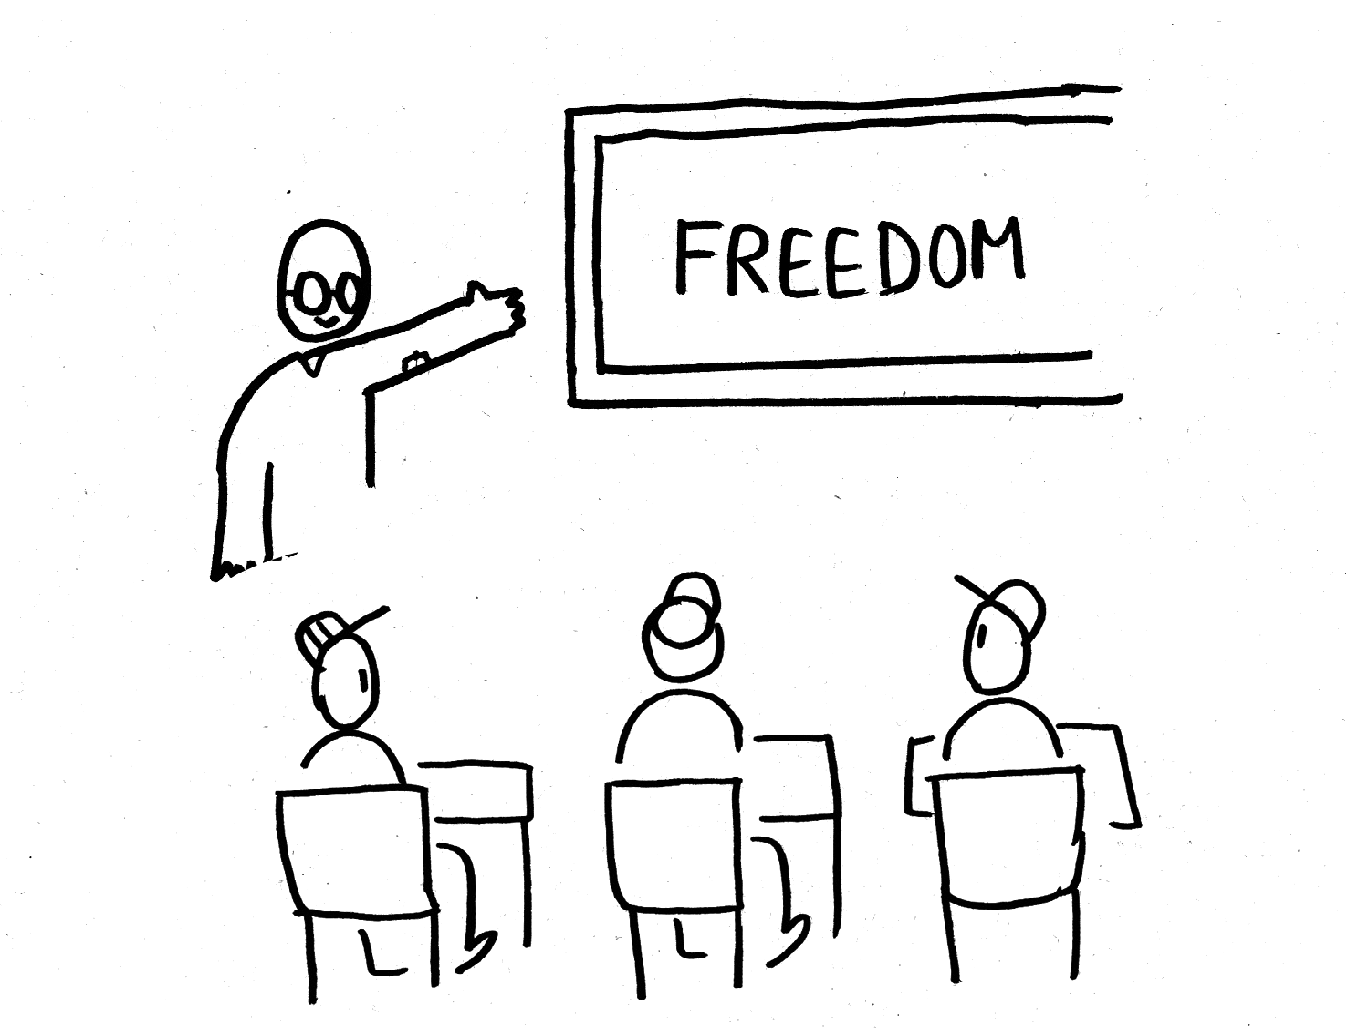
\includegraphics[scale=0.4]{fs-class}
  \end{figure}
\end{frame}

\begin{frame}
  \begin{figure}
    \centering
    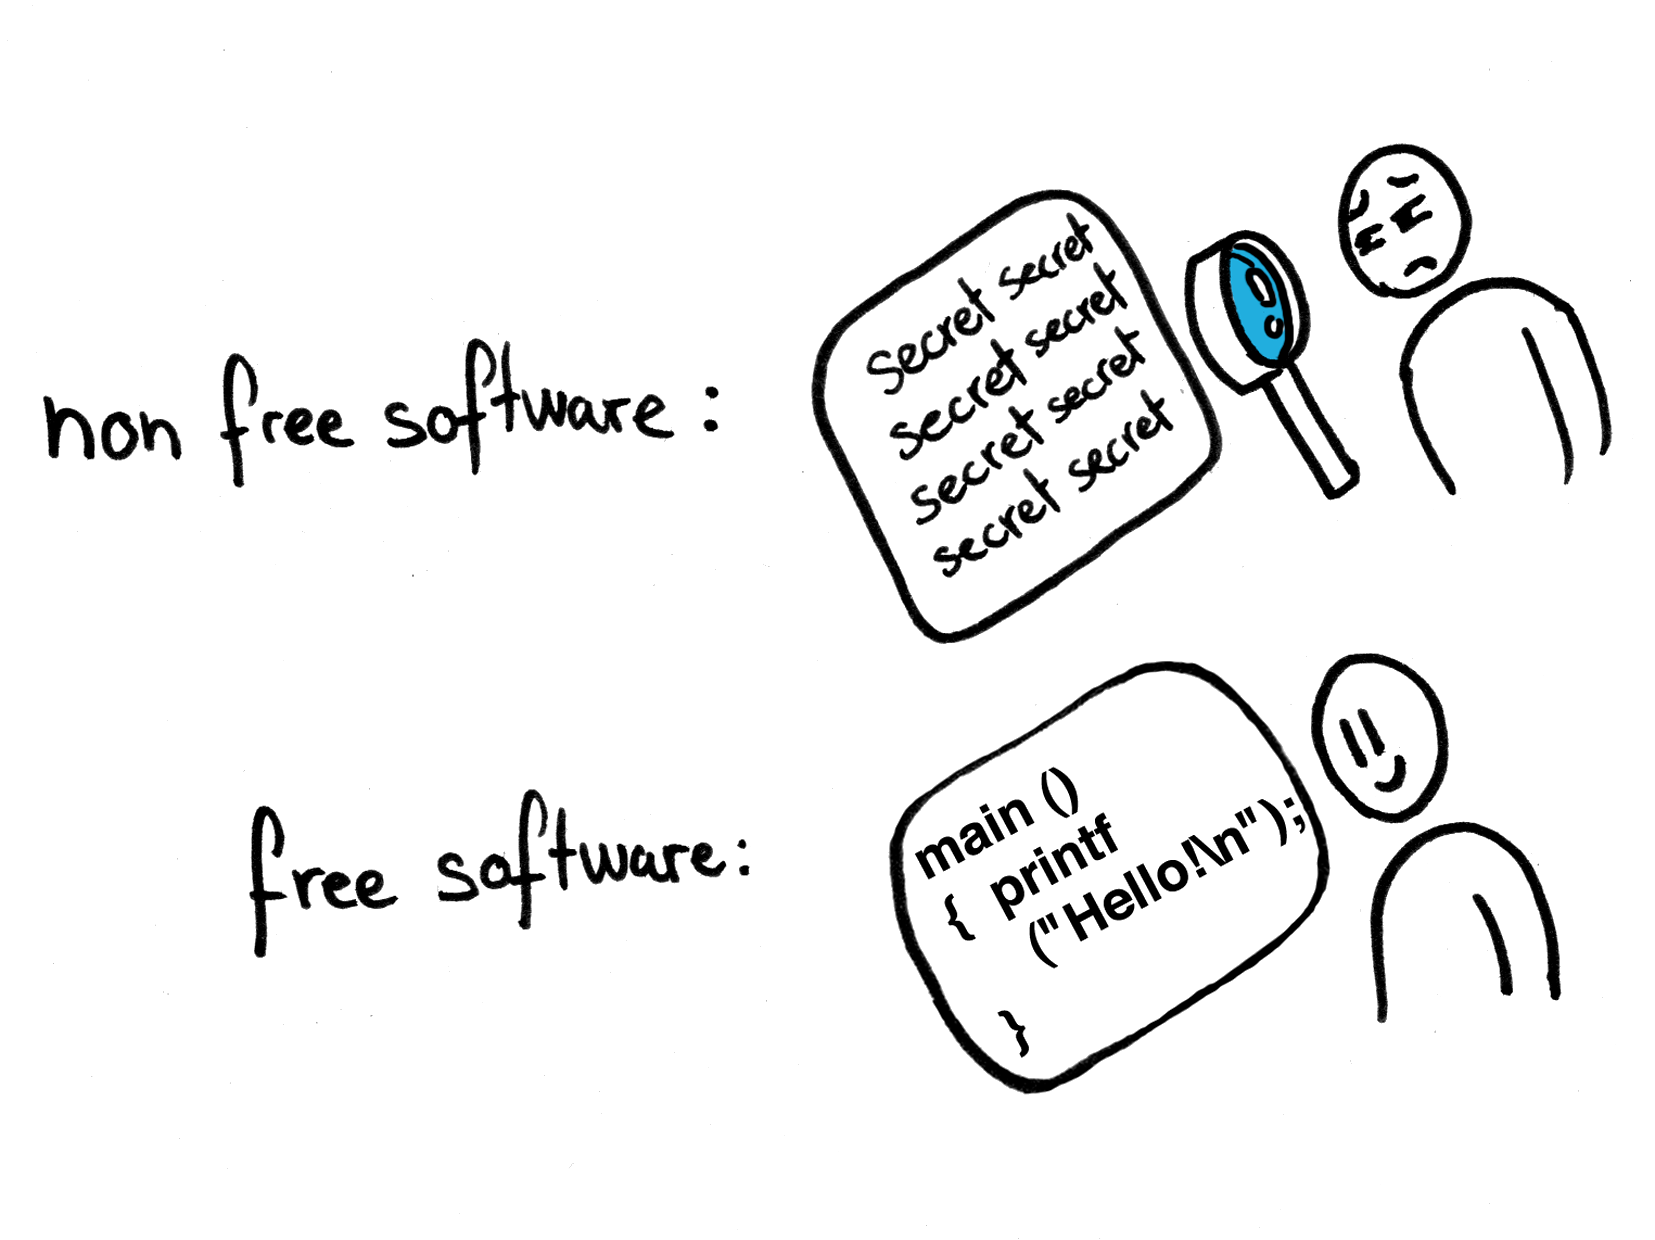
\includegraphics[scale=0.2]{kids-programmer}
  \end{figure}
\end{frame}

\begin{frame}
  \begin{figure}
    \centering
    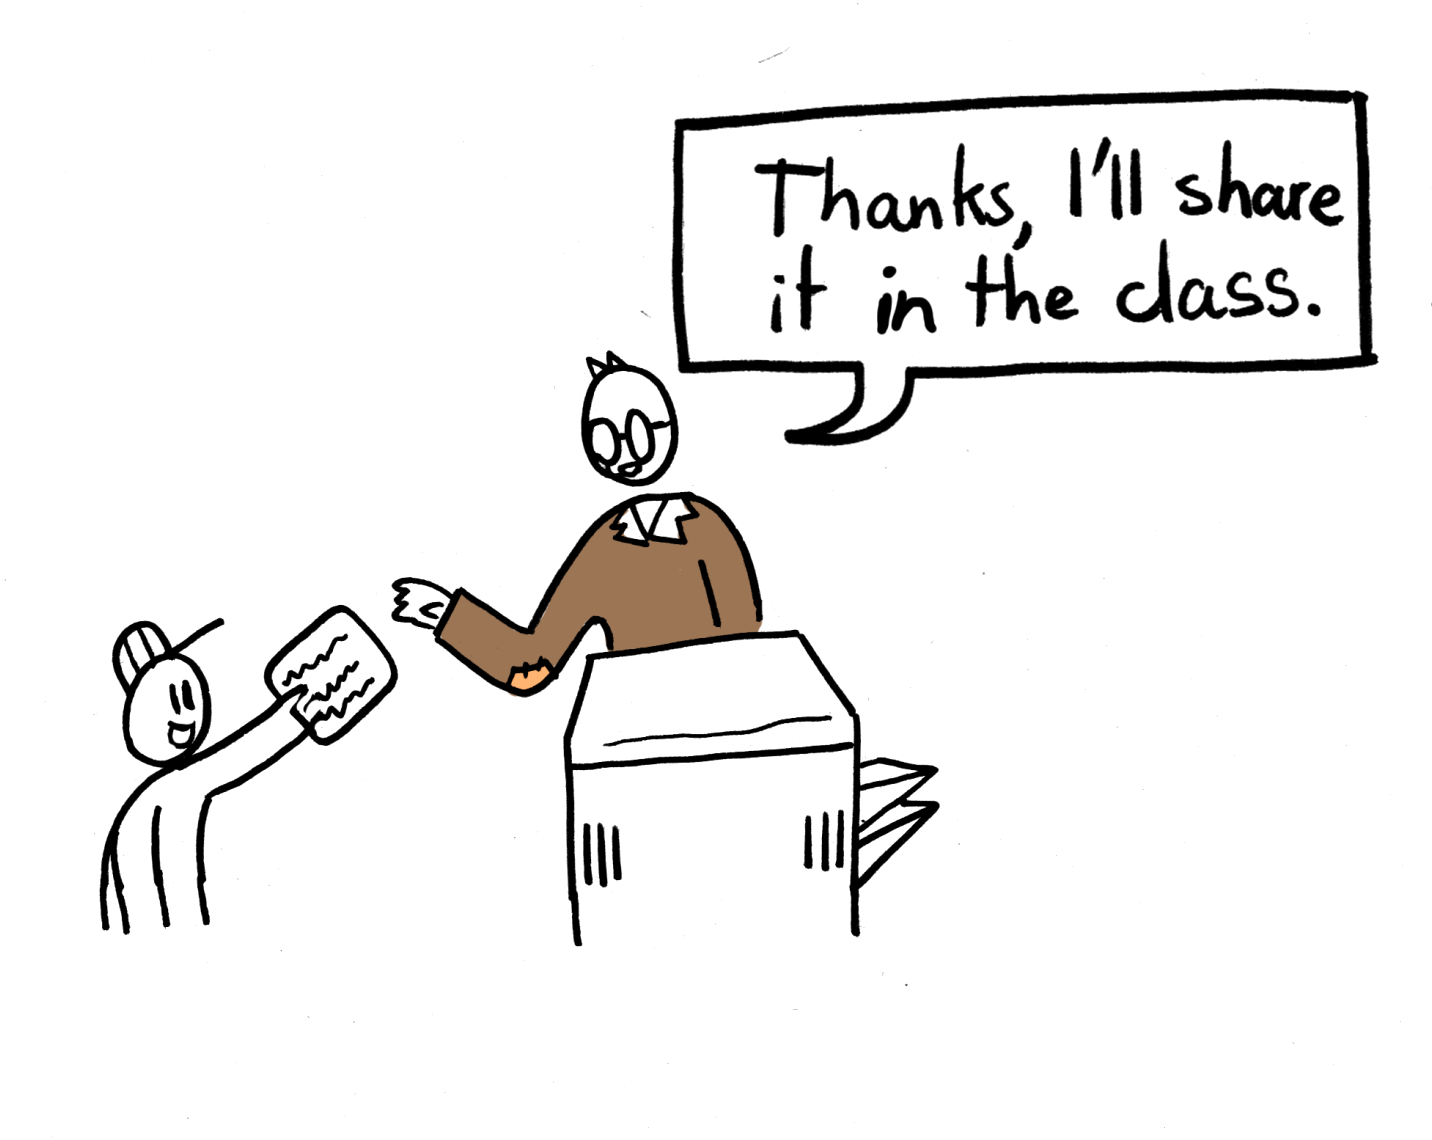
\includegraphics[scale=0.5]{teach-goodwill}
  \end{figure}
\end{frame}

\begin{frame}
  \begin{figure}
    \centering
    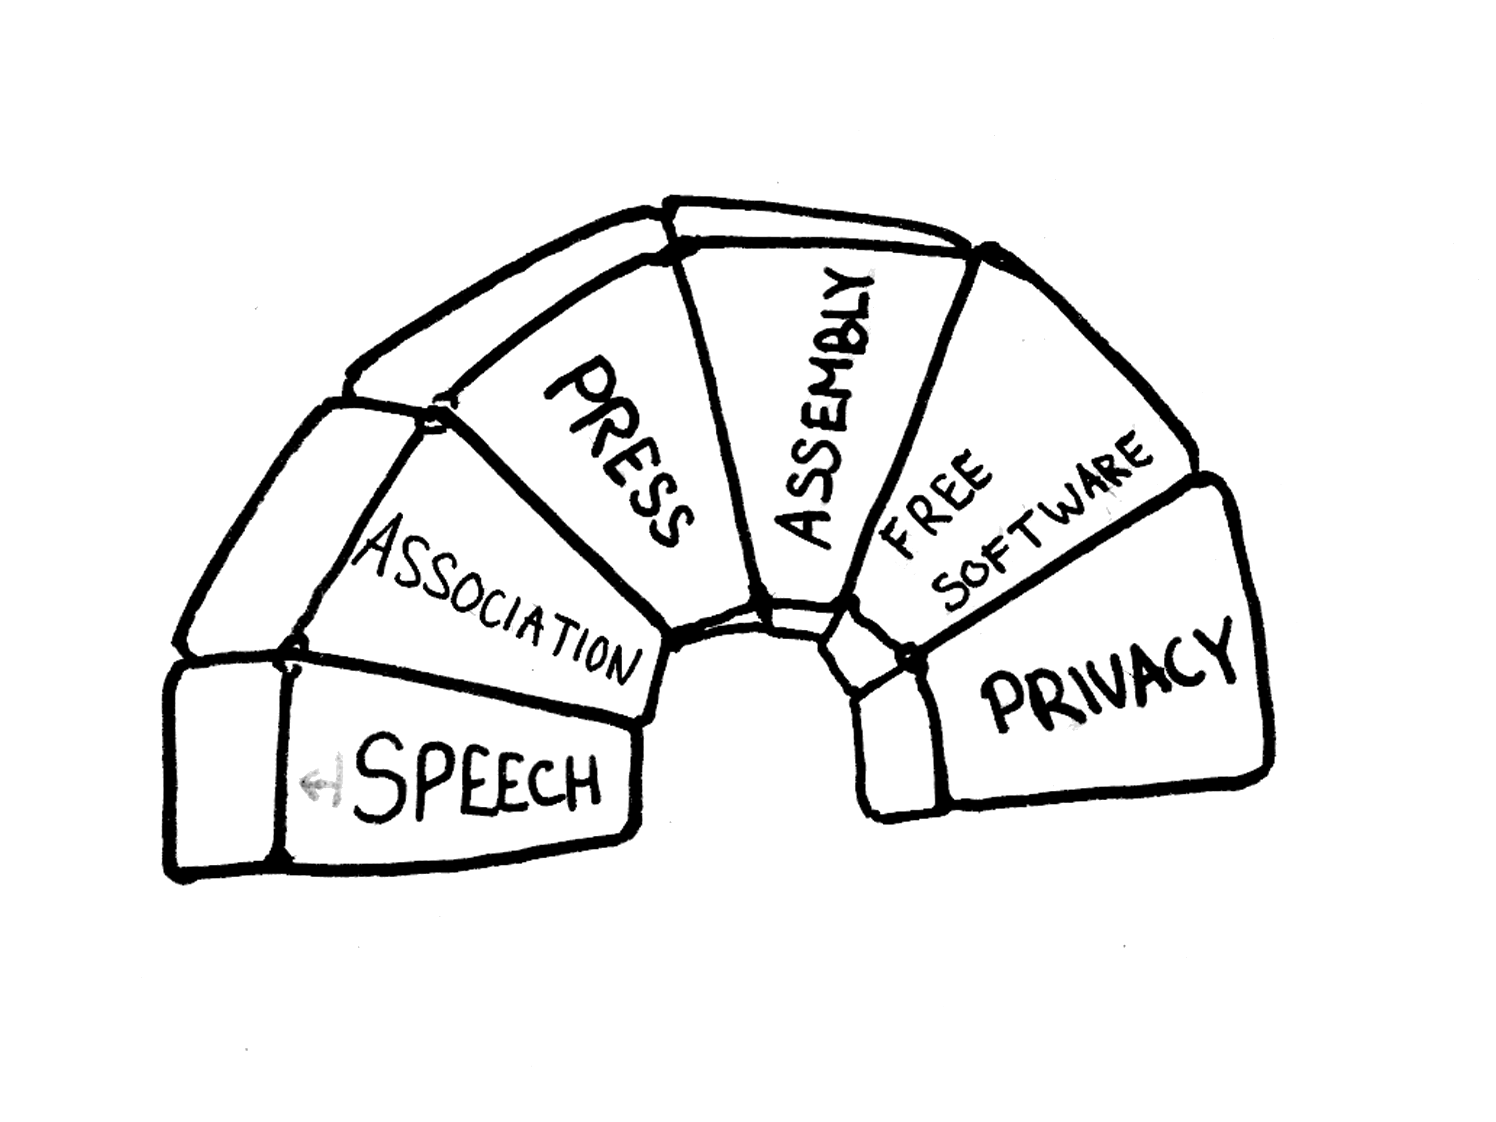
\includegraphics[scale=0.8]{life-rocks}
  \end{figure}
\end{frame}

\begin{frame}
  \frametitle{Last}
  \begin{itemize}[<+-+>]
  \item Untuk semua
  \item Kolaborasi, bukan persaigan
  \item Tanggung jawab untuk membantu dan mengajari
    bukan merasa lebih baik dan merendahkan.
  \item Mudah di hubungi
  \end{itemize}
\end{frame}

% 1
% \note{anyone know FS ?.}
\begin{frame}
  \begin{center}
    \Huge Senang bisa membantu.
  \end{center}
\end{frame}


\end{document}
